
\newpage
\section*{\LARGE Supplementary materials for ``Bayesian Fairness''}

\setcounter{section}{0}
%\setcounter{theorem}{0}

~\\

\section{Impossibility result}

\begin{theorem}\label{thm:impossible}
Calibration and balance conditions cannot hold simultaneously, except: (i) if there exists perfect decision rules that there exists $a,y$ s.t. $ P_\param^\pol(y\mid a) = 0 $ or $ P_\param^\pol(a\mid y) = 0 $, or (ii) $z$ is independent of $y$ that for each $z$, $ P_\param^\pol(z|y) \equiv \text{const.},~\forall y$.
\end{theorem}
\begin{proof}
We prove by contradiction. Using Bayes rule we first have
\begin{align}
    P_\param^\pol(a, z \mid y) =     P_\param^\pol(y, z \mid a) \cdot \frac{P_\param^\pol(a \mid y)}{P_\param^\pol(y \mid a)} ~.\label{eqn:1}
\end{align}
Suppose calibration condition holds, that is 
\[
P_\param^\pol(y, z \mid a) = P_\param^\pol(y \mid a) P_\param^\pol(z \mid a)
\]
Plug above into Eqn. (\ref{eqn:1}) we have 
\begin{align*}
    P_\param^\pol(a, z \mid y) &=    P_\param^\pol(y \mid a) P_\param^\pol(z \mid a) \cdot \frac{P_\param^\pol(a \mid y)}{P_\param^\pol(y \mid a)} \\
    &=P_\param^\pol(z \mid a) \cdot P_\param^\pol(a \mid y).
    \end{align*}
    On the other hand, if balanced condition holds too, we have
    \begin{align*}
    P_\param^\pol(a, z \mid y) =P_\param^\pol(a \mid y) \cdot P_\param^\pol(z \mid y) 
    \end{align*}
    Together we have that 
    \[
  P_\param^\pol(z \mid a) \cdot P_\param^\pol(a \mid y)  = P_\param^\pol(a \mid y) \cdot P_\param^\pol(z \mid y) \rightarrow   P_\param^\pol(z \mid a) =P_\param^\pol(z \mid y),
    \]
    which does not hold when condition (ii) does not hold, completing the proof. 
\end{proof}

~\\

\section{Trivial decision rules for balance}
\label{sec:counterexample}
 
\begin{theorem}
  A trivial decision rule of the form $\pol(a \mid x) = p_a$ can always satisfy balance for a Bayesian decision problem. However, it may be the only balanced decision rule, even when a non-trivial balanced policy can be found for every possible $\param \in \Param$.
  \label{lem:trivial-balance}
\end{theorem}
\begin{proof}
  For the first part, notice that Eqn. \eqref{eq:balanced-rule}
  can be always satisfied trivially if $\pol(a \mid x) = p_a$, i.e. we ignore the observations when taking our actions.
  For the second part, we can rewrite Eqn. \eqref{eq:balanced-rule} as
  \begin{align*}
    \sum_x \pol(a | x) \left[P_\theta(x, z | y) - P_\theta(x | y) P_\theta(z | y) \right] &= 0\\
    \sum_x \pol(a | x) \Delta_\theta(x, y, z) &= 0,
  \end{align*}
  where the $\Delta$ term is only dependent on the parameters.  This
  condition can be satisfied in two ways: the first is if the model
  $\param$ makes $x, z$ conditionally independent on $y$. The second
  is if the vector $\pol(a \mid \cdot)$ is orthogonal to
  $\Delta_\param(\cdot, y, z)$. If $|\CX| > |\CY \times \CZ|$, then,
  for any $\param$, we can always find a policy vector
  $\pol(a \mid \cdot)$ that is orthogonal to all vectors
  $\Delta_\param(\cdot, y, z)$. However, if these vectors across $\param$ have exactly degree of freedom being 1 (since they add up to 0, thus the rank of them can be at most the full rank - 1), then no single policy can be orthogonal
  to all, as otherwise the degree of freedom for this set of vectors will be at least 2. 
\end{proof}


\begin{example}
  In this balance example, there are two models. In the first model, for some value $y$, we have:
  \begin{align}
    P_{\param}(x=0|y) &= 1/4, &
                                P_{\param}(x=0|y,z=1) &= 1/4 - \epsilon, \\
    P_{\param}(x=1|y) &= 1/4, &
                                P_{\param}(x=1|y,z=1) &= 1/4 + \epsilon, \\
    P_{\param}(x=2|y) &= 1/4, &
                                P_{\param}(x=2|y,z=1) &= 1/4 + \epsilon, \\
  \end{align}
  so that
  \begin{align}
    P_{\param}(x=0|y) -  P_{\param}(x=0|y,z=1) &= \epsilon, \\
    P_{\param}(x=1|y) - P_{\param}(x=1|y,z=1) &=  - \epsilon\\
    P_{\param}(x=2|y) - P_{\param}(x=2|y,z=1) &=  - \epsilon
  \end{align}
  Similarly, we can construct models $\param'$ and $\param''$ so that the corresponding differences are $(-\epsilon, \epsilon, -\epsilon)$ and $(\epsilon, \epsilon, -\epsilon)$.
  For any policy $\pol(a \mid x)$ consider the vector $\pol_a = (\pol(a = 1 \mid x))_{x=1}^3$. Note that we can make the policy orthogonal to the first model simply by setting $\pol_a = (1/2, 1/2, 1)$.
\end{example}

~\\

\section{Proof of Theorem \ref{noise:model}}
\begin{proof}
We show the proof for Bayes-balance condition, while the proof for Marginal-balance resembles similarities. Denote the $(1-\delta)$-event that $\theta$ drawn from $\beta(\theta)$ that is $\epsilon$ close to the true model $\theta^*$ in all the conditional probabilities $P_{\theta}(x|y,z), P_{\theta}(x|y)$ as $\mathcal E$, then we have:
%\begin{align*}
%  &~~~\sum_x \pol(a | x)
%  \int_{\mathrlap{\Param }}
%    \left[P_\param(x, z | y)
%  - P_\param(x | y) P_\param(z | y) \right] \\
%  &=\int_{\theta \in \mathcal E} \sum_x \pol(a | x)
%    \left[P_{\param}(x, z | y)
%  - P_{\param}(x | y) P_{\param}(z | y) \right]\\
%  &+  \int_{\theta \notin \mathcal E}\sum_x \pol(a | x) \left[P_\param(x, z | y)
%  - P_\param(x | y) P_\param(z | y) \right] \\
% & \leq \int_{\theta \in \mathcal E} \sum_x \pol(a | x)
%    \left[P_{\param^*}(x, z | y)
%  - P_{\param^*}(x | y) P_{\param^*}(z | y) \right] +2\epsilon\\
%  &+\int_{\theta \notin \mathcal E}\sum_x \pol(a | x) \left[P_{\param^*}(x, z | y)
%  - P_{\param^*}(x | y) P_{\param^*}(z | y) \right] + 2\delta\\
%&  \leq \alpha+2(\epsilon+\delta).% \alpha \sum_x \pol(a | x) = \alpha.
%\end{align*}
\begin{align*}
  &~~~~~\bigl|\sum_x \pol(a | x)
    \left[P_{\param^*}(x, z | y)
  - P_{\param^*}(x | y) P_{\param^*}(z | y) \right]\bigr|\\
  &= \biggl|\int_{\theta \in \mathcal E} \sum_x \pol(a | x)
    \left[P_{\param^*}(x, z | y)
  - P_{\param^*}(x | y) P_{\param^*}(z | y) \right]\\
  &+\int_{\theta \notin \mathcal E}\sum_x \pol(a | x) \left[P_{\param^*}(x, z | y)
  - P_{\param^*}(x | y) P_{\param^*}(z | y) \right]\biggr|\\
  &\leq \biggl|\int_{\theta \in \mathcal E} \sum_x \pol(a | x)
    \left[P_{\param}(x, z | y)
  - P_{\param}(x | y) P_{\param}(z | y) \right] +2\epsilon\\
  &+\int_{\theta \notin \mathcal E}\sum_x \pol(a | x) \left[P_{\param^*}(x, z | y)
  - P_{\param}(x | y) P_{\param}(z | y) \right] + 2\delta\biggr|\\
  &\le \bigl |\sum_x \pol(a | x)
  \int_{\mathrlap{\Param }}
    \left[P_\param(x, z | y)
  - P_\param(x | y) P_\param(z | y) \right]\bigr| +  2(\epsilon+\delta).
  \end{align*}
  Summing over all $a,y,z$ gives us the results. 
\end{proof}
~\\

\section{Gradient calculations for optimal balance decision}
\label{sec:gradient}

For simplicity, let us define the vector in $\Simplex^{\CA}$:
\[
c_w(y,z) = \sum_x \pol_w(\cdot \mid x) \Delta(x, y, z),
\]
so that
\[
f_\lambda(w) = \util(\bel, \pol_w) -  \lambda \sum_{y,z} c_w(y,z)^\top c_w(y,z).
\]
Now
\begin{align*}
  &~~~~\grad_w \left(c_w(y,z)^\top c_w(y,z)\right)
  \\
  &= 
  \grad_w \sum_a c_w(y,z)_a^2\\
  &= 
  \sum_a 2 c_w(y,z)_a
  \grad_w c_w(y, z)_a
  \\
  \grad_w & c_w(y, z)_a
  = 
    \sum_x \grad_w \pol_w(a \mid x) \Delta(x, y, z),
\end{align*}
while
\begin{align}
  \grad \util(\bel, \pol_w)
  &=
    \int_\CX \dd \Pr_\bel(x) \grad_w \pol_w(a \mid x) \E_\bel (\util \mid x, a) 
\end{align}
Combining the two terms, we have
\begin{align*}
  \grad_w f_\lambda(w)
  &= 
    \int_\CX \grad_w \pol_w(a \mid x)
    \bigl[
    \dd \Pr_\bel(x) \E_\bel(U \mid x, a)
  \\
  &- 2 \lambda \sum_{y,z} c_w(y, z)_a \Delta(x, y, z) \dd \Lambda(x),
    \bigr].
\end{align*}
where $\Lambda$ is the Lebesgue measure.
We now derive the gradient for the $\grad_w \pol_w$ term. We consider
two parameterizations.
\paragraph{Independent policy parameters.} When $\pol(a \mid x) = w_{ax}$, we obtain
$$\partial \pol(a' \mid x') / \partial ax = \ind{ax = a'x'}$$.
This unfortunately requires projecting the policy parameters back to  the simplex. For this reason, it might be better to use a parameterization that allows unconstrained optimization. 
\paragraph{Softmax policy parameters.} When 
$$\pol(a \mid x) = e^{w_{ax}} / \sum_{a'} e^{w_{a'x}},$$
we have the following gradients:
\begin{align*}
  \partial \pol(a \mid x) / \partial ax
  &= 
    e^{w_{ax}} \sum_{a' \neq a} e^{w_{a'x}} \left(\sum_{a'} e^{w_{a'x}}\right)^{-2}
  \\
  \partial \pol(a \mid x) / \partial a'x
  &= 
    e^{w_{ax} + w_{a'x}}\left(\sum_{a''} e^{w_{a''x}}\right)^{-2}, ~ a \neq a'\\
  \partial \pol(a \mid x) / \partial a'x'
  &= 
    0, ~ ax \neq a'x'.
\end{align*}

~\\


\section{Empirical formulation.}
For infinite $\CX$, it may be more efficient to rewrite
\eqref{eq:balanced-bayes-constraint} as
\begin{align}
  0
  &=
    \int_{\CX} \pol(a \mid x) 
    \dd \left[ P(x, z \mid y)
    - P(x \mid y) P(z \mid y)\right]
  \\
  &= 
    \int_{\CX} \pol(a \mid x) 
    \left[ P(z \mid y, x)
    - P(z \mid y)\right] \dd P(x \mid y)\\
  &=
    \int_{\CX} \pol(a \mid x) 
    \left[ P(z \mid y, x)
    - P(z \mid y)\right] \frac{P(y \mid x)}{P(y)} \dd P(x)\\
  &\approx
    \sum_{x \sim P_\param(x)} \pol(a \mid x) 
    \left[ P(z \mid y, x)
    - P(z \mid y)\right] \frac{P(y \mid x)}{P(y)}
\intertext{simplifying by dropping the $P(y)$ term:}
  0 &\approx
    \sum_{x \sim P_\param(x)} \pol(a \mid x) 
    \left[ P(z \mid y, x)
    - P(z \mid y)\right] P(y \mid x),
\end{align}
This allows us to approximate the integral by sampling $x$, and can be
useful for e.g. regression problems.

\section{Complete figures}
This section has complete versions of the figures which could not fit in the main text.
\begin{figure*}
\centering
 \subfloat[$\lambda=0$]{
   % This file was created by matlab2tikz.
%
%The latest updates can be retrieved from
%  http://www.mathworks.com/matlabcentral/fileexchange/22022-matlab2tikz-matlab2tikz
%where you can also make suggestions and rate matlab2tikz.
%
\definecolor{mycolor1}{rgb}{0.00000,0.75000,0.75000}%
%
\begin{tikzpicture}

\begin{axis}[%
width=0.951\fwidth,
height=0.75\fwidth,
at={(0\fwidth,0\fwidth)},
scale only axis,
xmode=log,
xmin=1,
xmax=100,
xminorticks=true,
xlabel={t},
ymin=4.5,
ymax=8,
ylabel={$U,F$},
axis background/.style={fill=white}
]
\addplot [color=blue, line width=2.0pt, forget plot]
  table[row sep=crcr]{%
1	5.43561523059217\\
2	5.90370595362012\\
3	5.86193877425643\\
4	6.1974251447707\\
5	6.37538745144895\\
6	6.29084098710727\\
7	6.37533818756081\\
8	6.50213010808347\\
9	6.5991724386949\\
10	6.52046523295858\\
11	6.72543938736623\\
12	6.79086221447693\\
13	6.73720035131321\\
14	6.73338708212267\\
15	6.72543680895541\\
16	6.69340595276163\\
17	6.7374401920428\\
18	6.76459636329051\\
19	6.81917107124367\\
20	6.81961739074537\\
21	6.80848937741292\\
22	6.76496273549776\\
23	6.81943224558462\\
24	6.82707956663492\\
25	6.82513922838762\\
26	6.80872080097762\\
27	6.8194279261825\\
28	6.8189260277632\\
29	6.80836851035401\\
30	6.80853114441057\\
31	6.81931954445528\\
32	6.73856115284411\\
33	6.73816264740434\\
34	6.73350236577814\\
35	6.70687112292105\\
36	6.6785416628419\\
37	6.67686803452494\\
38	6.73847232580075\\
39	6.81942547936638\\
40	6.82688492791769\\
41	6.82666694620967\\
42	6.82685885290022\\
43	6.82704019063763\\
44	6.82689924230517\\
45	6.82677823960367\\
46	6.8270597587393\\
47	6.8194560097514\\
48	6.82689843014005\\
49	6.82701602901863\\
50	6.82681169930566\\
51	6.81949797532045\\
52	6.82669354234299\\
53	6.81943329511497\\
54	6.82651491512469\\
55	6.82704770792639\\
56	6.82679743590289\\
57	6.82658758155496\\
58	6.82669828218253\\
59	6.82660948782845\\
60	6.82669798274291\\
61	6.8265894448791\\
62	6.82677142197074\\
63	6.82681491374407\\
64	6.82666114793132\\
65	6.80855816288338\\
66	6.81943481045244\\
67	6.82660396672482\\
68	6.82386355702123\\
69	6.81947471789097\\
70	6.82700074175287\\
71	6.82693449357647\\
72	6.82709850214994\\
73	6.82660499877464\\
74	6.82697649873285\\
75	6.82670593695921\\
76	6.82675415174255\\
77	6.82687238452097\\
78	6.82695391513762\\
79	6.82698434483159\\
80	6.82686631929662\\
81	6.82688791087935\\
82	6.82646811164595\\
83	6.82644252014829\\
84	6.82665183718036\\
85	6.82669758685249\\
86	6.82676665652696\\
87	6.82695751973057\\
88	6.82658946086894\\
89	6.82655885737069\\
90	6.82664771118609\\
91	6.82677188302957\\
92	6.82669723134228\\
93	6.82649131899508\\
94	6.82694362296807\\
95	6.82701100800417\\
96	6.82689276186491\\
97	6.82697942973237\\
98	6.8265959260873\\
99	6.82685566499548\\
100	6.82661794251553\\
};
\addplot [color=black!50!green, dashed, line width=3.0pt, forget plot]
  table[row sep=crcr]{%
1	5.41383459952623\\
2	6.03977740818528\\
3	6.34445896962323\\
4	6.36360081485984\\
5	6.5327140246455\\
6	6.54312011538435\\
7	6.60180812138142\\
8	6.73373741924754\\
9	6.73566894837812\\
10	6.79427286043087\\
11	6.79651547742057\\
12	6.81745557776205\\
13	6.82361089403465\\
14	6.82453008513155\\
15	6.81832088322606\\
16	6.78744690174988\\
17	6.8245307167606\\
18	6.82360223044389\\
19	6.82320123869577\\
20	6.82664800772996\\
21	6.82680811620926\\
22	6.82647925470442\\
23	6.82692086547104\\
24	6.8269265759928\\
25	6.82693425257449\\
26	6.8268229060682\\
27	6.82700552417735\\
28	6.82667175358748\\
29	6.82668179704755\\
30	6.82696045898621\\
31	6.82660833511297\\
32	6.82680589726841\\
33	6.82671589421294\\
34	6.82682294359754\\
35	6.82701707308604\\
36	6.82650493640409\\
37	6.82699220517708\\
38	6.82668021066387\\
39	6.82672209879424\\
40	6.82681624339904\\
41	6.82673440179816\\
42	6.82689211021934\\
43	6.82677720152432\\
44	6.82694542985608\\
45	6.82666056532852\\
46	6.82671478552557\\
47	6.82693547661731\\
48	6.82672478318047\\
49	6.82677490664466\\
50	6.82656216462366\\
51	6.82648634438907\\
52	6.82704568401014\\
53	6.826862274337\\
54	6.82707378292588\\
55	6.82701064453263\\
56	6.82655872230876\\
57	6.82680284995162\\
58	6.82675484205814\\
59	6.82669898677491\\
60	6.8269587402534\\
61	6.82659491807925\\
62	6.8270850859566\\
63	6.82673295666194\\
64	6.82699550615579\\
65	6.82685223576769\\
66	6.82671348441515\\
67	6.82673202844262\\
68	6.82712820153405\\
69	6.82689184429809\\
70	6.82683272593571\\
71	6.82648201507614\\
72	6.82674866309257\\
73	6.82671747591638\\
74	6.82699024215261\\
75	6.82717941910823\\
76	6.82694493886605\\
77	6.8267239335274\\
78	6.82696730470131\\
79	6.82694340122485\\
80	6.82682976358288\\
81	6.82660119141053\\
82	6.82686412764447\\
83	6.82699084765003\\
84	6.8267722735916\\
85	6.82674429780571\\
86	6.82694302876559\\
87	6.82675714405635\\
88	6.82696031751509\\
89	6.82689255300199\\
90	6.82702023326717\\
91	6.82696488326549\\
92	6.82660850972417\\
93	6.8268004525055\\
94	6.82679611886495\\
95	6.82682594191007\\
96	6.82686735298234\\
97	6.82672601577022\\
98	6.82680403091386\\
99	6.82704486981606\\
100	6.8267221923614\\
};
\addplot [color=red, dashdotted, line width=2.0pt, forget plot]
  table[row sep=crcr]{%
1	4.65679844872143\\
2	5.69596508675862\\
3	6.12283278302887\\
4	6.64373241409889\\
5	7.32558978567296\\
6	6.08163155109078\\
7	6.19748304313167\\
8	6.87388547503056\\
9	7.08389848708165\\
10	7.66590296789734\\
11	7.53380043435034\\
12	7.62021550620541\\
13	6.55198691005539\\
14	7.31957601971931\\
15	7.35795487617778\\
16	6.56844918258317\\
17	6.60268271810485\\
18	6.93824349667414\\
19	6.54115540687113\\
20	6.91918785115645\\
21	7.21517127808337\\
22	7.13583366054737\\
23	6.66321201520444\\
24	6.98638303153576\\
25	6.78324605322824\\
26	7.38817377199521\\
27	6.63843044254195\\
28	6.75672123473148\\
29	7.3764343870945\\
30	7.19570861786257\\
31	6.65820831042757\\
32	6.9430024004874\\
33	6.85869875035141\\
34	6.84454259485917\\
35	6.98880616760368\\
36	7.08431244310177\\
37	7.25857722575256\\
38	6.98686399745706\\
39	6.6537099802175\\
40	6.7214629047179\\
41	6.57818486200004\\
42	6.78856195660524\\
43	6.98657442393879\\
44	6.70851618145228\\
45	6.77231060119333\\
46	6.91138081525664\\
47	6.80900520532078\\
48	6.8955319793459\\
49	6.84792233580796\\
50	6.79275017251076\\
51	6.71426555740713\\
52	6.59004662459356\\
53	6.77652926179091\\
54	6.65083295234543\\
55	6.85126864447383\\
56	6.74854673311024\\
57	6.75003213226614\\
58	6.89126758286218\\
59	6.82121018801547\\
60	6.73429925858514\\
61	6.55866795761166\\
62	6.77542717061313\\
63	6.7505053995152\\
64	6.61001242197726\\
65	7.25454977658437\\
66	6.66630203216666\\
67	6.49701316241904\\
68	6.74842532476086\\
69	6.71504163949096\\
70	6.97439204366755\\
71	6.76367082195242\\
72	6.96309910967014\\
73	6.82447935225019\\
74	6.97808966701071\\
75	6.92487707804123\\
76	6.66720140412107\\
77	6.79555773655483\\
78	6.8885209752185\\
79	6.82374109038333\\
80	6.72908264481633\\
81	6.86784379199626\\
82	6.63745368452247\\
83	6.5131420448435\\
84	6.88807751914145\\
85	6.72286398044753\\
86	6.73792752347492\\
87	6.93224164162795\\
88	6.837553331591\\
89	6.70329794971067\\
90	6.77161494678466\\
91	6.92391725886576\\
92	6.64034499050567\\
93	6.80661355109981\\
94	6.90661745847731\\
95	6.90906010305707\\
96	6.73117108750913\\
97	6.96005426572143\\
98	6.54290590591496\\
99	6.69200091471541\\
100	6.67305945104694\\
};
\addplot [color=mycolor1, dotted, line width=3.0pt, forget plot]
  table[row sep=crcr]{%
1	4.63856673683556\\
2	7.65090449353503\\
3	7.29720941968353\\
4	6.39411547781226\\
5	5.59180859447572\\
6	5.91103616867134\\
7	5.65345033980548\\
8	6.99157334254097\\
9	6.98378088352546\\
10	6.36878678535445\\
11	6.5703513033626\\
12	6.72120527280937\\
13	7.18827355673923\\
14	7.07400805356152\\
15	7.07676946422607\\
16	6.68918545343691\\
17	6.87716882988162\\
18	7.21295461204102\\
19	6.89059757703387\\
20	6.6418700279056\\
21	6.72969261054924\\
22	6.58527483721895\\
23	6.84422565408741\\
24	6.76291708398274\\
25	6.78586446833003\\
26	6.97929349712728\\
27	6.91929251936603\\
28	6.59430908038756\\
29	6.82168411870536\\
30	6.86077963582398\\
31	6.71389518734896\\
32	6.78498708606475\\
33	6.79899086704355\\
34	6.85315001850439\\
35	6.96486748159995\\
36	6.73627790220896\\
37	6.8592233857706\\
38	6.56505333926661\\
39	6.73635246282633\\
40	6.75269318472154\\
41	6.67726773578806\\
42	6.90187689510759\\
43	6.78042022470713\\
44	6.77019613843506\\
45	6.73856118706226\\
46	6.57185409950028\\
47	6.96761071311978\\
48	6.66130453339595\\
49	6.80708379997048\\
50	6.85748230435172\\
51	6.70135826348809\\
52	6.9938569734353\\
53	6.72539117699799\\
54	6.94640793627233\\
55	6.9385051726723\\
56	6.61631698807355\\
57	6.788520931626\\
58	6.88572558664489\\
59	6.68380106971717\\
60	6.86253282851936\\
61	6.65810790284873\\
62	6.8793638877059\\
63	6.78922309796063\\
64	6.94456473813911\\
65	6.70260082131938\\
66	6.72230045188807\\
67	6.69964002067404\\
68	7.00732110672733\\
69	6.81079303773709\\
70	6.68424630783847\\
71	6.52353247112277\\
72	6.73012734112837\\
73	6.69496855949307\\
74	6.92703451903552\\
75	7.02396178656437\\
76	6.81686683630093\\
77	6.59425523559705\\
78	6.95528299863492\\
79	6.75296627805458\\
80	6.78184138131174\\
81	6.63659860007914\\
82	6.88566575528246\\
83	6.92879059314807\\
84	6.64710033562532\\
85	6.65151555001541\\
86	6.9180522788148\\
87	6.71736971916958\\
88	6.90775109592753\\
89	6.89321397542376\\
90	6.80705343437269\\
91	6.93499379578587\\
92	6.59613086758874\\
93	6.86088232672981\\
94	6.67935174396831\\
95	6.81958814386339\\
96	6.78885095717227\\
97	6.62347677209479\\
98	6.66807026959861\\
99	6.99366307038507\\
100	6.7131226265173\\
};
\end{axis}
\end{tikzpicture}%
  }
  \subfloat[$\lambda=0.25$]{
    % This file was created by matlab2tikz.
%
%The latest updates can be retrieved from
%  http://www.mathworks.com/matlabcentral/fileexchange/22022-matlab2tikz-matlab2tikz
%where you can also make suggestions and rate matlab2tikz.
%
\definecolor{mycolor1}{rgb}{0.00000,0.75000,0.75000}%
%
\begin{tikzpicture}

\begin{axis}[%
width=0.951\fwidth,
height=0.75\fwidth,
at={(0\fwidth,0\fwidth)},
scale only axis,
xmode=log,
xmin=1,
xmax=100,
xminorticks=true,
xlabel={t},
ylabel={$U, F$},
ymin=3,
ymax=8,
axis background/.style={fill=white}
]
\addplot [color=blue, line width=2.0pt, forget plot]
  table[row sep=crcr]{%
1	5.48092030379997\\
2	5.62187002690099\\
3	5.95863155946218\\
4	6.28898882529671\\
5	6.37263646084564\\
6	6.44619863535187\\
7	6.51978070369432\\
8	6.6260112803707\\
9	6.59969215942956\\
10	6.64710138462075\\
11	6.64739151299339\\
12	6.64510042770851\\
13	6.64152382540431\\
14	6.77898626490996\\
15	6.78942211106642\\
16	6.78461368559541\\
17	6.78747870326049\\
18	6.78938642097554\\
19	6.78832161718462\\
20	6.78775050690658\\
21	6.78944722876843\\
22	6.78917577314025\\
23	6.78819139814796\\
24	6.78724347966865\\
25	6.78821620436663\\
26	6.78831214850696\\
27	6.7880922368358\\
28	6.7881723236791\\
29	6.78794233482332\\
30	6.78813814586129\\
31	6.78820354351858\\
32	6.78841099428386\\
33	6.78808353541935\\
34	6.7881908225767\\
35	6.78774827696057\\
36	6.7885187243922\\
37	6.78845419838743\\
38	6.78814836495893\\
39	6.78821228904136\\
40	6.78818735684172\\
41	6.78799405430338\\
42	6.7882713816731\\
43	6.78927591624498\\
44	6.78946030227827\\
45	6.78821020841118\\
46	6.78827185230104\\
47	6.78860337850886\\
48	6.78748352584787\\
49	6.78799354670293\\
50	6.78842672785986\\
51	6.7880902860153\\
52	6.78808388647639\\
53	6.78747738661796\\
54	6.78819916095484\\
55	6.78835895289234\\
56	6.78843293590063\\
57	6.78825725240079\\
58	6.78829796145325\\
59	6.788057466024\\
60	6.78839237562291\\
61	6.78834851740735\\
62	6.78735253906824\\
63	6.78775411240988\\
64	6.78863576035963\\
65	6.78755861187669\\
66	6.78954119015546\\
67	6.78873337301612\\
68	6.78816033804725\\
69	6.78820344967906\\
70	6.78776361064147\\
71	6.78814177015364\\
72	6.7879366996741\\
73	6.7880936081835\\
74	6.78825561226921\\
75	6.78821316644409\\
76	6.78918787026003\\
77	6.78818333235925\\
78	6.78819645711209\\
79	6.78810751942358\\
80	6.78842982644288\\
81	6.78739048420254\\
82	6.78823104668009\\
83	6.78781609618644\\
84	6.78820734692313\\
85	6.78828044289443\\
86	6.78722601773148\\
87	6.78755406937019\\
88	6.78811157856524\\
89	6.78808107645364\\
90	6.789012996106\\
91	6.7881650039973\\
92	6.78821720889247\\
93	6.78807168410838\\
94	6.78810800021703\\
95	6.78793379320975\\
96	6.78826043758827\\
97	6.78807781437123\\
98	6.78818537206819\\
99	6.78850763801694\\
100	6.7884621883911\\
};
\addplot [color=black!50!green, dashed, line width=3.0pt, forget plot]
  table[row sep=crcr]{%
1	5.46839092366965\\
2	5.75703558072284\\
3	6.21187308663476\\
4	6.39102664381444\\
5	6.55586234089632\\
6	6.38413615637934\\
7	6.42300581162868\\
8	6.67498693237809\\
9	6.63039319016224\\
10	6.58773391003488\\
11	6.75296577578321\\
12	6.786443793693\\
13	6.78805569029723\\
14	6.78745585366746\\
15	6.78832428887165\\
16	6.78830066490763\\
17	6.78839106970021\\
18	6.78808802788535\\
19	6.78798694582777\\
20	6.78817693494755\\
21	6.7881008909547\\
22	6.78842032667698\\
23	6.78783128904056\\
24	6.78875615083487\\
25	6.78845727850269\\
26	6.78819401413074\\
27	6.78834196285126\\
28	6.7872101033022\\
29	6.7879980507075\\
30	6.78824430728795\\
31	6.78816970586208\\
32	6.78818801908122\\
33	6.78814017664448\\
34	6.78825078323049\\
35	6.7881484859051\\
36	6.78818691493551\\
37	6.78808987102091\\
38	6.78816298338296\\
39	6.78799846176474\\
40	6.78828094214078\\
41	6.78727871939925\\
42	6.78803975010666\\
43	6.78725571301125\\
44	6.78871518089493\\
45	6.78840508970577\\
46	6.7875707596091\\
47	6.7881728716072\\
48	6.78846952964538\\
49	6.78817772400779\\
50	6.78840021851439\\
51	6.78822370152359\\
52	6.78740754507343\\
53	6.78818214694285\\
54	6.78826729796029\\
55	6.78794709000275\\
56	6.78819769453097\\
57	6.78773687436855\\
58	6.78760780764942\\
59	6.78820024812653\\
60	6.78822638564773\\
61	6.78816361161253\\
62	6.78832451810031\\
63	6.78840398227284\\
64	6.78810379421081\\
65	6.7882192655374\\
66	6.7882812746018\\
67	6.78767994390469\\
68	6.78789414506478\\
69	6.78833152743326\\
70	6.78812570838307\\
71	6.78853051769768\\
72	6.78820591270197\\
73	6.78840134179175\\
74	6.78833646862341\\
75	6.78714175770295\\
76	6.78827649125506\\
77	6.78761416139175\\
78	6.78818828234791\\
79	6.78820835330531\\
80	6.78869172117444\\
81	6.78888773725641\\
82	6.78807839890497\\
83	6.78822911534438\\
84	6.7882605284278\\
85	6.78824522127325\\
86	6.78813733439761\\
87	6.78828150957633\\
88	6.787818875421\\
89	6.78808023524246\\
90	6.78808690828464\\
91	6.78820378585089\\
92	6.78810395152641\\
93	6.78826222843939\\
94	6.78821516715624\\
95	6.7884244130633\\
96	6.78815086989971\\
97	6.78823200461007\\
98	6.78762008169212\\
99	6.78764861589493\\
100	6.78759288324044\\
};
\addplot [color=red, dashdotted, line width=2.0pt, forget plot]
  table[row sep=crcr]{%
1	3.95263838270111\\
2	3.82503765619641\\
3	4.69915687329073\\
4	4.95179395517991\\
5	5.69532493678198\\
6	5.37334301528087\\
7	4.83235868797524\\
8	4.73554152570934\\
9	5.01931591636941\\
10	5.03432141135122\\
11	4.79254541499617\\
12	4.63914092183212\\
13	4.44750001169128\\
14	4.81685316598652\\
15	4.9147788424582\\
16	4.91327394352937\\
17	4.95995623494322\\
18	4.8945337204222\\
19	4.84879148065828\\
20	4.83909002285821\\
21	4.88259365579378\\
22	4.88389090533673\\
23	4.8443938066954\\
24	4.83840179753397\\
25	4.84558816878397\\
26	4.84905292663818\\
27	4.84147078022581\\
28	4.84372820754065\\
29	4.83890505616955\\
30	4.84232199646838\\
31	4.84523950410094\\
32	4.85078354779625\\
33	4.84135735710565\\
34	4.84520888873435\\
35	4.84215081653731\\
36	4.85535850522084\\
37	4.85185247997884\\
38	4.84260169610015\\
39	4.84620634763515\\
40	4.84523575187968\\
41	4.83902567068879\\
42	4.84701671196802\\
43	4.87609116537311\\
44	4.88206656252824\\
45	4.84539564610091\\
46	4.84731781906082\\
47	4.85657048784665\\
48	4.84464814453533\\
49	4.84034483610184\\
50	4.85098637586876\\
51	4.85234480413716\\
52	4.84223427910482\\
53	4.83645625338907\\
54	4.84534540433531\\
55	4.84989668463203\\
56	4.85152070699286\\
57	4.84710109351825\\
58	4.84850862271226\\
59	4.8417612393451\\
60	4.8505172651455\\
61	4.84854018635913\\
62	4.84166599328614\\
63	4.83795694229326\\
64	4.85812270662427\\
65	4.8507748368422\\
66	4.88437423777575\\
67	4.85926481587375\\
68	4.84382853660602\\
69	4.8450886394879\\
70	4.83777595797139\\
71	4.8436077111013\\
72	4.83723787081233\\
73	4.8419858580276\\
74	4.84700191788378\\
75	4.84679719167575\\
76	4.88422845265261\\
77	4.84492363174228\\
78	4.84542290433572\\
79	4.84308012880218\\
80	4.85170602717477\\
81	4.84406941230317\\
82	4.84661435851207\\
83	4.83788327052865\\
84	4.84567275514356\\
85	4.84723479294532\\
86	4.83903092538253\\
87	4.83854193953482\\
88	4.84165658956618\\
89	4.84096009660066\\
90	4.86812900077183\\
91	4.84417172920604\\
92	4.84595715415907\\
93	4.84059852688428\\
94	4.84207974058152\\
95	4.84058822114876\\
96	4.84739615953176\\
97	4.84066509683728\\
98	4.84408611041905\\
99	4.85435432738002\\
100	4.85140753714343\\
};
\addplot [color=mycolor1, dotted, line width=3.0pt, forget plot]
  table[row sep=crcr]{%
1	4.43942617049761\\
2	6.07517227920279\\
3	6.01511546400837\\
4	7.99001185146673\\
5	6.91853861731467\\
6	7.45736885559621\\
7	5.9696968988519\\
8	5.90044821555372\\
9	6.53253989933909\\
10	5.95793744141482\\
11	4.47853828240861\\
12	5.01187651983101\\
13	4.86994172661999\\
14	4.87457926082996\\
15	4.91605950930105\\
16	4.83664217269984\\
17	4.84487405751951\\
18	4.84572345362514\\
19	4.84496677844009\\
20	4.84859591315895\\
21	4.8439187330126\\
22	4.85436336951604\\
23	4.84095204112765\\
24	4.86334743088784\\
25	4.85229857867871\\
26	4.84514781002158\\
27	4.84965309635877\\
28	4.83928916416435\\
29	4.84189589312187\\
30	4.84704232748438\\
31	4.84549575927436\\
32	4.84486903809857\\
33	4.84236622368815\\
34	4.84766997345754\\
35	4.85758994431681\\
36	4.84579416567247\\
37	4.84096626422101\\
38	4.84505804961238\\
39	4.8440266791363\\
40	4.84775057449601\\
41	4.84209322722535\\
42	4.84050324640196\\
43	4.83980167280306\\
44	4.85923425685094\\
45	4.85111829634059\\
46	4.84132164675338\\
47	4.84370161642999\\
48	4.87223462946916\\
49	4.84432618495737\\
50	4.8500961427862\\
51	4.84586521700634\\
52	4.84466882674989\\
53	4.84385534411402\\
54	4.84618282826888\\
55	4.85639560861603\\
56	4.8456548959247\\
57	4.84125063954534\\
58	4.84248664382494\\
59	4.84531192138565\\
60	4.84571944195174\\
61	4.84383104434909\\
62	4.84870278970119\\
63	4.85126878016323\\
64	4.84210931804219\\
65	4.84625260846576\\
66	4.84761300621132\\
67	4.83951697497941\\
68	4.84891722764123\\
69	4.84990546659528\\
70	4.84234548798647\\
71	4.85552485686154\\
72	4.84534656853895\\
73	4.85214524633418\\
74	4.84833846211763\\
75	4.83836834799854\\
76	4.84747334309443\\
77	4.84577873600088\\
78	4.84566127923588\\
79	4.84656159051625\\
80	4.85932831037586\\
81	4.86458441816834\\
82	4.84154805775504\\
83	4.84631576231663\\
84	4.84721937222264\\
85	4.8458013115131\\
86	4.84218017264925\\
87	4.84713277748063\\
88	4.83723898611049\\
89	4.84187774364254\\
90	4.84171840375588\\
91	4.8452678398018\\
92	4.84182079956507\\
93	4.84699098516083\\
94	4.84549640548173\\
95	4.85158555409688\\
96	4.84409812448365\\
97	4.84640282767493\\
98	4.84023191773009\\
99	4.83639997556977\\
100	4.83899503618132\\
};
\end{axis}
\end{tikzpicture}%
  }
  \subfloat[$\lambda=0.5$]{
    % This file was created by matlab2tikz.
%
%The latest updates can be retrieved from
%  http://www.mathworks.com/matlabcentral/fileexchange/22022-matlab2tikz-matlab2tikz
%where you can also make suggestions and rate matlab2tikz.
%
\definecolor{mycolor1}{rgb}{0.00000,0.75000,0.75000}%
%
\begin{tikzpicture}

\begin{axis}[%
width=0.951\fwidth,
height=0.75\fwidth,
at={(0\fwidth,0\fwidth)},
scale only axis,
xmode=log,
xmin=1,
xmax=100,
xminorticks=true,
xlabel={t},
ymin=2,
ymax=7,
axis background/.style={fill=white}
]
\addplot [color=blue, line width=2.0pt, forget plot]
  table[row sep=crcr]{%
1	5.43626321740328\\
2	5.62955957449209\\
3	5.83892212841107\\
4	6.08455180148673\\
5	6.45389213646402\\
6	6.51404201900693\\
7	6.55425288332807\\
8	6.47841299626561\\
9	6.62069875641757\\
10	6.51422248577047\\
11	6.59838520559784\\
12	6.59032275016397\\
13	6.52849619086474\\
14	6.68240075733416\\
15	6.70628180193069\\
16	6.70366440054659\\
17	6.70078300565614\\
18	6.70264005866184\\
19	6.70272040838255\\
20	6.70215960026927\\
21	6.7035515874975\\
22	6.70405002626636\\
23	6.70380004965903\\
24	6.70280860477349\\
25	6.70188832548547\\
26	6.70154419712915\\
27	6.70290303559077\\
28	6.70099710415468\\
29	6.70193379267451\\
30	6.70120150981987\\
31	6.70173152738914\\
32	6.70159866600691\\
33	6.70148331010774\\
34	6.70024700158092\\
35	6.70162388648996\\
36	6.70122567452083\\
37	6.70119760380918\\
38	6.7008942387301\\
39	6.70207192686816\\
40	6.70206106174765\\
41	6.70118803780591\\
42	6.7011708537815\\
43	6.70121592271\\
44	6.70090701893929\\
45	6.70090952627623\\
46	6.70172791977211\\
47	6.7004604519536\\
48	6.70214417070081\\
49	6.70087927793523\\
50	6.7009280299354\\
51	6.70192571875951\\
52	6.70171886250275\\
53	6.70150820728044\\
54	6.70126159777429\\
55	6.70041242169488\\
56	6.7002853540649\\
57	6.70046583835858\\
58	6.70020648356859\\
59	6.70116548685459\\
60	6.70050519866534\\
61	6.7015615201992\\
62	6.7007685612289\\
63	6.70095050594716\\
64	6.70154935714809\\
65	6.70152349860255\\
66	6.70070897977991\\
67	6.7009292344296\\
68	6.70068914149036\\
69	6.70163551712463\\
70	6.70142476387294\\
71	6.70069739926064\\
72	6.7017336129983\\
73	6.70128008473107\\
74	6.70162543894496\\
75	6.70146658599244\\
76	6.70170456840915\\
77	6.7013768002497\\
78	6.70182944797324\\
79	6.70116360226985\\
80	6.701438682881\\
81	6.70092732271296\\
82	6.70135911617293\\
83	6.70188062229687\\
84	6.70075474316751\\
85	6.70097329900569\\
86	6.70040857565787\\
87	6.70120199869424\\
88	6.70120379847468\\
89	6.70170383955328\\
90	6.70113156603443\\
91	6.70058910840515\\
92	6.70055443379444\\
93	6.70091509145021\\
94	6.70170584002308\\
95	6.70130045964099\\
96	6.70227846487977\\
97	6.70187435109027\\
98	6.70119790741984\\
99	6.70133993723436\\
100	6.70064902183277\\
};
\addplot [color=black!50!green, dashed, line width=3.0pt, forget plot]
  table[row sep=crcr]{%
1	5.51006868459902\\
2	5.94349925651812\\
3	6.15110188956242\\
4	6.02712399624356\\
5	6.32392569534522\\
6	6.36115851019674\\
7	6.36007362082859\\
8	6.42304614951736\\
9	6.46234178919198\\
10	6.46733988080431\\
11	6.45899027408367\\
12	6.3374431395461\\
13	6.54985803215858\\
14	6.3167027540054\\
15	6.46001002676741\\
16	6.56942958143311\\
17	6.61343634104224\\
18	6.63292515036324\\
19	6.63448250199397\\
20	6.63488106426994\\
21	6.63474315974286\\
22	6.68991621855335\\
23	6.6335990864829\\
24	6.69904685642871\\
25	6.70141875769818\\
26	6.7012806526023\\
27	6.70070437469069\\
28	6.70101301806078\\
29	6.70067654491554\\
30	6.70099908199053\\
31	6.70110335421526\\
32	6.70109454031283\\
33	6.70048011400453\\
34	6.70015802246409\\
35	6.70146803260837\\
36	6.70137519147395\\
37	6.70074615877402\\
38	6.70091163421494\\
39	6.7008946179437\\
40	6.70109518272528\\
41	6.70205145033657\\
42	6.70115273392061\\
43	6.70186718313822\\
44	6.70177380992648\\
45	6.7003804780666\\
46	6.70153952966726\\
47	6.70174797129619\\
48	6.70057765354134\\
49	6.70081922974977\\
50	6.70164333602487\\
51	6.70125515905557\\
52	6.70152742403787\\
53	6.70163646612874\\
54	6.70157301629276\\
55	6.701414269396\\
56	6.70151509569165\\
57	6.70113067220305\\
58	6.70067348960663\\
59	6.70094302840244\\
60	6.70066241369534\\
61	6.70171037678393\\
62	6.7017258902379\\
63	6.70100013577623\\
64	6.70084519318045\\
65	6.70123086292297\\
66	6.70103013736592\\
67	6.70117679885823\\
68	6.70136115786824\\
69	6.70167814502445\\
70	6.70122192741145\\
71	6.70183309433243\\
72	6.70100999249549\\
73	6.70135356970916\\
74	6.7002459876897\\
75	6.70146912361473\\
76	6.70130258398882\\
77	6.70075589014854\\
78	6.70080348452352\\
79	6.70112183391194\\
80	6.70120314765165\\
81	6.70119447031542\\
82	6.70144475842244\\
83	6.70137848453271\\
84	6.70168043308462\\
85	6.70077627802382\\
86	6.70071854612631\\
87	6.70101623736037\\
88	6.70104533420828\\
89	6.70135513010366\\
90	6.70056144078923\\
91	6.70102557689087\\
92	6.7006300362861\\
93	6.70107085890124\\
94	6.70153290457477\\
95	6.70133276766025\\
96	6.70119862303415\\
97	6.70089139040385\\
98	6.70152026042981\\
99	6.70007620915822\\
100	6.70036852816079\\
};
\addplot [color=red, dashdotted, line width=2.0pt, forget plot]
  table[row sep=crcr]{%
1	2.44661771734869\\
2	2.52576353700595\\
3	2.16127647791958\\
4	3.0310290948882\\
5	3.40887425643453\\
6	3.50341814626276\\
7	3.56683307706032\\
8	3.73648862770094\\
9	3.23565565554268\\
10	3.40502086781842\\
11	3.04321944910621\\
12	3.01889669235785\\
13	3.43068866230066\\
14	3.25900115565335\\
15	3.17273095025148\\
16	3.10459827121771\\
17	3.0526650791918\\
18	3.09139487891992\\
19	3.09579296675206\\
20	3.09234915988499\\
21	3.09851430049847\\
22	3.10488187422497\\
23	3.11031833793038\\
24	3.09025546200949\\
25	3.07799538254974\\
26	3.05651836407002\\
27	3.09294115326098\\
28	3.04643784169409\\
29	3.08269460708509\\
30	3.07199875153622\\
31	3.06343319656065\\
32	3.07375106751663\\
33	3.06639676553553\\
34	3.05995126777791\\
35	3.07517841982544\\
36	3.06389299412385\\
37	3.06951122517533\\
38	3.04740118393345\\
39	3.08209796772388\\
40	3.07641205413439\\
41	3.05399563766818\\
42	3.05893438157334\\
43	3.05541018738379\\
44	3.06393384924717\\
45	3.04896819364968\\
46	3.07750178838152\\
47	3.05587980147252\\
48	3.08182658514786\\
49	3.04540555034994\\
50	3.06253296378515\\
51	3.07015540037389\\
52	3.06967956686681\\
53	3.0665229029738\\
54	3.06112004082199\\
55	3.05154570012539\\
56	3.04896094300526\\
57	3.05485326870482\\
58	3.04000064341995\\
59	3.059682219609\\
60	3.06316955979892\\
61	3.06141679688057\\
62	3.04373363846218\\
63	3.06791502934542\\
64	3.0757031610305\\
65	3.07958268848526\\
66	3.05845004880157\\
67	3.06552120542576\\
68	3.0419291877304\\
69	3.06806252792471\\
70	3.06832192190414\\
71	3.05477491131693\\
72	3.06448088366623\\
73	3.04826170050289\\
74	3.06948504914674\\
75	3.06412523565948\\
76	3.07259231360712\\
77	3.06403226648865\\
78	3.06970412697863\\
79	3.06165521805732\\
80	3.0614821477698\\
81	3.052753008387\\
82	3.06648346891204\\
83	3.07741163270134\\
84	3.04639913183469\\
85	3.06273214783606\\
86	3.06596710461126\\
87	3.04983966925001\\
88	3.06539272911671\\
89	3.06856762532641\\
90	3.05256539118647\\
91	3.03999612848695\\
92	3.05343433068084\\
93	3.05168086156649\\
94	3.06665063702698\\
95	3.05274503115123\\
96	3.08200349747352\\
97	3.07318177136839\\
98	3.06615315275989\\
99	3.05534532007844\\
100	3.05738636915808\\
};
\addplot [color=mycolor1, dotted, line width=3.0pt, forget plot]
  table[row sep=crcr]{%
1	5.10841690753339\\
2	6.30366720328818\\
3	6.59816030254869\\
4	6.17790900319201\\
5	4.46475981640557\\
6	5.00765820609084\\
7	4.30951390227002\\
8	4.04161842546795\\
9	4.01485656248218\\
10	4.34312892872975\\
11	3.66541471620045\\
12	3.517951425459\\
13	3.61233274197403\\
14	3.74518751805426\\
15	4.16236954544025\\
16	3.64187637079015\\
17	3.4741715491685\\
18	3.29478144435632\\
19	3.18876107018515\\
20	3.20397854482619\\
21	3.19320600929792\\
22	3.27036325372438\\
23	3.20516039434347\\
24	3.05980848849459\\
25	3.05167931384347\\
26	3.05717743757322\\
27	3.0412954175818\\
28	3.06149776452893\\
29	3.04849873207019\\
30	3.04518142355283\\
31	3.05500058612968\\
32	3.05073964570803\\
33	3.05686069870436\\
34	3.04945434987303\\
35	3.07163211580473\\
36	3.07857793419349\\
37	3.07135457940943\\
38	3.05417963349527\\
39	3.06161284949563\\
40	3.07797428607014\\
41	3.08166389658056\\
42	3.06906824068655\\
43	3.07685730044911\\
44	3.06959642640651\\
45	3.04382768227879\\
46	3.06171377644948\\
47	3.07010403124248\\
48	3.05731202400714\\
49	3.07062597924447\\
50	3.06229126911754\\
51	3.05690352916751\\
52	3.06922983803813\\
53	3.05873407555027\\
54	3.0560740176733\\
55	3.0796699396199\\
56	3.05903847571533\\
57	3.05346016169011\\
58	3.05274905852315\\
59	3.06334635906267\\
60	3.05083683979572\\
61	3.06929869363696\\
62	3.07363736785062\\
63	3.06771725206619\\
64	3.0555037122552\\
65	3.06363688025101\\
66	3.05429921537096\\
67	3.05786906562215\\
68	3.06089932774921\\
69	3.08142837576992\\
70	3.07119110837081\\
71	3.07819963661889\\
72	3.07592939418843\\
73	3.06934163009663\\
74	3.04161092943315\\
75	3.06115524034447\\
76	3.05413353643378\\
77	3.04342239143652\\
78	3.06695751758088\\
79	3.06223131468353\\
80	3.06790529182809\\
81	3.07235109327085\\
82	3.06559871297931\\
83	3.06886571268794\\
84	3.07193206572329\\
85	3.06176523652693\\
86	3.05312708109413\\
87	3.05450888405249\\
88	3.0615663512455\\
89	3.05752676840432\\
90	3.05975652143678\\
91	3.07211379467446\\
92	3.0525903118369\\
93	3.04773333165863\\
94	3.06121170064906\\
95	3.06467535806715\\
96	3.07540315101183\\
97	3.06243086424018\\
98	3.06862373610331\\
99	3.04294148478522\\
100	3.05839878495847\\
};
\end{axis}
\end{tikzpicture}%
  }
  \\
  \subfloat[$\lambda=0.75$]{
    % This file was created by matlab2tikz.
%
%The latest updates can be retrieved from
%  http://www.mathworks.com/matlabcentral/fileexchange/22022-matlab2tikz-matlab2tikz
%where you can also make suggestions and rate matlab2tikz.
%
\definecolor{mycolor1}{rgb}{0.00000,0.75000,0.75000}%
%
\begin{tikzpicture}

\begin{axis}[%
width=0.951\fwidth,
height=0.75\fwidth,
at={(0\fwidth,0\fwidth)},
scale only axis,
xmode=log,
xmin=1,
xmax=100,
xminorticks=true,
xlabel={t},
ymin=0,
ymax=7,
ylabel={$U, F$},
axis background/.style={fill=white}
]
\addplot [color=blue, line width=2.0pt, forget plot]
  table[row sep=crcr]{%
1	5.47461127098968\\
2	5.60478890856896\\
3	5.77191033058464\\
4	5.90011496868576\\
5	6.14377790957163\\
6	6.31041948276384\\
7	6.43552914365433\\
8	6.5151531251348\\
9	6.54729734736349\\
10	6.57798495912498\\
11	6.57849571632306\\
12	6.58765985244295\\
13	6.58900819766999\\
14	6.58807470034135\\
15	6.58544669469427\\
16	6.58533577780727\\
17	6.58370067428244\\
18	6.58971365581165\\
19	6.5878980368345\\
20	6.59048092832187\\
21	6.59125044154283\\
22	6.5896710150567\\
23	6.58987286386257\\
24	6.58946117658065\\
25	6.58999333445314\\
26	6.59031718167873\\
27	6.59139413998349\\
28	6.59090165755066\\
29	6.59051023277067\\
30	6.59219941170473\\
31	6.59124669937017\\
32	6.58902226344559\\
33	6.58930522013265\\
34	6.59156801046039\\
35	6.59140118319131\\
36	6.59071800018758\\
37	6.5904962121109\\
38	6.58994289370681\\
39	6.59067144643273\\
40	6.5908473033638\\
41	6.58935869164842\\
42	6.59079752619829\\
43	6.59045257663437\\
44	6.59038156874226\\
45	6.58922214845872\\
46	6.5920430806679\\
47	6.59061552462121\\
48	6.5910853518908\\
49	6.5904707507656\\
50	6.59147532593014\\
51	6.59088905580135\\
52	6.59228441522875\\
53	6.59101992136476\\
54	6.59064064465195\\
55	6.59183783311411\\
56	6.59023817047242\\
57	6.59061017708232\\
58	6.5906193777462\\
59	6.59140530114315\\
60	6.5912579079603\\
61	6.59103059374945\\
62	6.59073429065668\\
63	6.5902464349662\\
64	6.59060596841733\\
65	6.59015307164583\\
66	6.59133709302133\\
67	6.59065526384808\\
68	6.58958255899406\\
69	6.59157679882054\\
70	6.59033990286414\\
71	6.59149880127007\\
72	6.59081749662089\\
73	6.58978538380844\\
74	6.59092637473552\\
75	6.58927529131999\\
76	6.58850343746042\\
77	6.59070961917545\\
78	6.59053467074177\\
79	6.58991848266028\\
80	6.59074090596838\\
81	6.59116797494771\\
82	6.59120811456219\\
83	6.58951958489378\\
84	6.59076403901614\\
85	6.58992010133594\\
86	6.59063253300245\\
87	6.59074681389064\\
88	6.59131520405029\\
89	6.58979941235916\\
90	6.58994888558284\\
91	6.59168176024839\\
92	6.59066396864525\\
93	6.59105539706456\\
94	6.59127950787074\\
95	6.59064023962094\\
96	6.59008138513551\\
97	6.59140183039189\\
98	6.58838036017117\\
99	6.5909343332388\\
100	6.59170125491083\\
};
\addplot [color=black!50!green, dashed, line width=3.0pt, forget plot]
  table[row sep=crcr]{%
1	5.62056595098105\\
2	5.9249699465451\\
3	6.01582827122022\\
4	5.95571514939206\\
5	5.92294247321893\\
6	5.81452251942304\\
7	6.13426812770014\\
8	6.04595676543718\\
9	6.29227294231064\\
10	6.27799612179181\\
11	6.32051997859251\\
12	6.36527532407389\\
13	6.32925991780952\\
14	6.45465237806581\\
15	6.58223240737318\\
16	6.57987442531153\\
17	6.55874072799058\\
18	6.5753041864462\\
19	6.58119554829056\\
20	6.58728407958621\\
21	6.57809056851983\\
22	6.56764059133101\\
23	6.41013588735602\\
24	6.38917378777253\\
25	6.58721628658142\\
26	6.58203616141645\\
27	6.4153585168044\\
28	6.56214565465418\\
29	6.42451672084935\\
30	6.57980421789207\\
31	6.59042602754726\\
32	6.59044529564649\\
33	6.59080569187187\\
34	6.59089611744954\\
35	6.58916534077888\\
36	6.59030181816158\\
37	6.59088695127249\\
38	6.58937832439878\\
39	6.59148671433531\\
40	6.59073721108426\\
41	6.59093404750414\\
42	6.59087742004054\\
43	6.58928541970452\\
44	6.59058564316579\\
45	6.59132828384597\\
46	6.59058851035584\\
47	6.59110263530547\\
48	6.59147553116448\\
49	6.58668393005854\\
50	6.59062363782734\\
51	6.59101515662169\\
52	6.59176251951947\\
53	6.58857868597947\\
54	6.59013423143927\\
55	6.59111909588808\\
56	6.5911457483472\\
57	6.59003852850639\\
58	6.59143982256265\\
59	6.59048536674524\\
60	6.59039176821099\\
61	6.59137154542976\\
62	6.5912535226034\\
63	6.58981582043099\\
64	6.5908918306807\\
65	6.59083300972301\\
66	6.59079121501016\\
67	6.59030883873119\\
68	6.59129857301594\\
69	6.59128229744416\\
70	6.59095332658505\\
71	6.59023081358638\\
72	6.59081865364851\\
73	6.59094026619255\\
74	6.59040142378658\\
75	6.59163684757572\\
76	6.59110676104285\\
77	6.59119701707623\\
78	6.58989897914213\\
79	6.5918191325617\\
80	6.59000392128006\\
81	6.59005624567473\\
82	6.59175293524183\\
83	6.5908999928299\\
84	6.59095496039431\\
85	6.58972726779356\\
86	6.59027090444657\\
87	6.59089103275845\\
88	6.59083663036135\\
89	6.59079717575128\\
90	6.59042755723988\\
91	6.59032670713473\\
92	6.59144685236426\\
93	6.5909022764905\\
94	6.59173282877921\\
95	6.58975668648628\\
96	6.58944811703204\\
97	6.5909704505714\\
98	6.58887279368135\\
99	6.59056883095371\\
100	6.59080516986559\\
};
\addplot [color=red, dashdotted, line width=2.0pt, forget plot]
  table[row sep=crcr]{%
1	0.962011577752915\\
2	1.39512833468571\\
3	1.90148489293405\\
4	1.51648055618043\\
5	2.15248666521931\\
6	1.55704328138457\\
7	1.66059810154288\\
8	1.52166767379182\\
9	1.60756285452165\\
10	1.57032375887657\\
11	1.57143632706561\\
12	1.54570012712595\\
13	1.53062124352496\\
14	1.54268502801898\\
15	1.53021067085092\\
16	1.55206916663035\\
17	1.54627922395726\\
18	1.51390174557473\\
19	1.50375418924415\\
20	1.51530747681262\\
21	1.52196737407071\\
22	1.50354898705708\\
23	1.51332011123504\\
24	1.52232901674692\\
25	1.52509841996306\\
26	1.52238627498701\\
27	1.5324730708447\\
28	1.51163420208493\\
29	1.51812829528253\\
30	1.52774156845851\\
31	1.52183786551656\\
32	1.5016521070917\\
33	1.49397777104937\\
34	1.51952082470017\\
35	1.52980925719026\\
36	1.52606705237248\\
37	1.52515602796127\\
38	1.50973845097226\\
39	1.52151282867688\\
40	1.53441438633646\\
41	1.52415222096287\\
42	1.51132177031528\\
43	1.5246991042189\\
44	1.50540365539768\\
45	1.50579300125202\\
46	1.5332974431763\\
47	1.52602816377732\\
48	1.52498943304033\\
49	1.52505167508116\\
50	1.52936828998447\\
51	1.52360673777914\\
52	1.53058250934036\\
53	1.52357239030125\\
54	1.52025395181835\\
55	1.53499050028086\\
56	1.51742772358661\\
57	1.51441659560209\\
58	1.51420820595266\\
59	1.5262997058346\\
60	1.53616242827644\\
61	1.52204501826377\\
62	1.51266612225863\\
63	1.5190132195052\\
64	1.52431344447975\\
65	1.51530419794324\\
66	1.52201531315481\\
67	1.51061899113799\\
68	1.51304669429054\\
69	1.52532175891914\\
70	1.53260170132874\\
71	1.52225905085154\\
72	1.50963037140345\\
73	1.52293726685294\\
74	1.52308518163793\\
75	1.4950927590338\\
76	1.50963368680608\\
77	1.51272511429317\\
78	1.51042633785373\\
79	1.50938242359903\\
80	1.5271682127886\\
81	1.5117185420591\\
82	1.52766007832391\\
83	1.51122470668482\\
84	1.51941129140273\\
85	1.51728704039085\\
86	1.52688068863037\\
87	1.50792216758675\\
88	1.51772700059157\\
89	1.51734457771922\\
90	1.51448813532051\\
91	1.53151859073494\\
92	1.52116535307287\\
93	1.51578575724323\\
94	1.52090562538418\\
95	1.51986831699292\\
96	1.50477239990879\\
97	1.52614502228845\\
98	1.4935503656753\\
99	1.51752656157145\\
100	1.53496968961844\\
};
\addplot [color=mycolor1, dotted, line width=3.0pt, forget plot]
  table[row sep=crcr]{%
1	4.6864935622248\\
2	4.8994383088347\\
3	4.56109313648738\\
4	4.90229035547094\\
5	2.9314300803944\\
6	3.2784332597462\\
7	2.46963199592331\\
8	2.30125152271061\\
9	2.01471564245944\\
10	2.17712372051914\\
11	1.78625426786003\\
12	1.85353123296186\\
13	1.99614342802232\\
14	1.65287461428729\\
15	1.49633284810289\\
16	1.48610098565703\\
17	1.45156396181048\\
18	1.47406316737917\\
19	1.46740662240884\\
20	1.50873895369633\\
21	1.45078965236607\\
22	1.45245977605543\\
23	1.71819478818221\\
24	2.08550862826438\\
25	1.5059355521904\\
26	1.47394259570511\\
27	1.75330416344819\\
28	1.38731873977995\\
29	1.70173662068909\\
30	1.46762136054097\\
31	1.50989567888606\\
32	1.52057424298062\\
33	1.52296770227207\\
34	1.51890013441686\\
35	1.51167634567613\\
36	1.52013496455013\\
37	1.53042250209518\\
38	1.51614460001237\\
39	1.51068803218364\\
40	1.52349879587756\\
41	1.5292094373918\\
42	1.52723516835788\\
43	1.50219367701738\\
44	1.50889764085272\\
45	1.53357949409282\\
46	1.5063426671682\\
47	1.52330362351915\\
48	1.52806722140564\\
49	1.48492641984674\\
50	1.50496302104093\\
51	1.51726658029489\\
52	1.51662375013351\\
53	1.48434709843271\\
54	1.51950876152417\\
55	1.51591219634932\\
56	1.52244113525343\\
57	1.51228811211186\\
58	1.51907869642937\\
59	1.52153657235561\\
60	1.52002671698928\\
61	1.52644490901635\\
62	1.51264572580944\\
63	1.5160114727441\\
64	1.52871982636947\\
65	1.52455740252168\\
66	1.52881396551966\\
67	1.52041366900985\\
68	1.51920423367879\\
69	1.52572400377125\\
70	1.52896228076713\\
71	1.50694486971597\\
72	1.5191129634431\\
73	1.53589170731109\\
74	1.51554168107362\\
75	1.52114588847516\\
76	1.5073119787335\\
77	1.53177729643885\\
78	1.49938469465641\\
79	1.52493589459921\\
80	1.51681359788873\\
81	1.50273815004913\\
82	1.53692226281642\\
83	1.51074892880607\\
84	1.53056388532285\\
85	1.52037492759945\\
86	1.51626804395327\\
87	1.5065737477751\\
88	1.52211768630356\\
89	1.52115051067854\\
90	1.521429717609\\
91	1.50829188644711\\
92	1.53568509407678\\
93	1.51780971278461\\
94	1.5267654175131\\
95	1.51765382436885\\
96	1.51725665471583\\
97	1.51173138823043\\
98	1.50648110697348\\
99	1.50703573590319\\
100	1.5100847459919\\
};
\end{axis}
\end{tikzpicture}%
  }
  \subfloat[$\lambda=1$]{
    % This file was created by matlab2tikz.
%
%The latest updates can be retrieved from
%  http://www.mathworks.com/matlabcentral/fileexchange/22022-matlab2tikz-matlab2tikz
%where you can also make suggestions and rate matlab2tikz.
%
\definecolor{mycolor1}{rgb}{0.00000,0.75000,0.75000}%
%
\begin{tikzpicture}

\begin{axis}[%
width=0.951\fwidth,
height=0.75\fwidth,
at={(0\fwidth,0\fwidth)},
scale only axis,
xmode=log,
xmin=1,
xmax=100,
xminorticks=true,
xlabel={t},
ymin=0,
ymax=6,
axis background/.style={fill=white}
]
\addplot [color=blue, line width=2.0pt, forget plot]
  table[row sep=crcr]{%
1	5.00968895853338\\
2	5.01867889787289\\
3	4.96734479517662\\
4	5.04284731151066\\
5	4.96410589090651\\
6	4.92855692547961\\
7	4.9849530218492\\
8	5.06366975530007\\
9	5.0646593325148\\
10	5.12795539320582\\
11	4.89537719631868\\
12	5.1613757241285\\
13	4.97670201742803\\
14	5.09142292366911\\
15	4.82148690792892\\
16	5.13409097540207\\
17	5.1341222403747\\
18	4.99850448319231\\
19	4.83165018984949\\
20	5.02222433844796\\
21	5.09962536428159\\
22	5.27934133662201\\
23	4.79337511133361\\
24	4.90405968430141\\
25	4.92075754330474\\
26	5.11674761478616\\
27	5.07383774437207\\
28	5.03240729832405\\
29	5.10667372816094\\
30	5.11074333496191\\
31	4.97878759507553\\
32	5.00046708761504\\
33	4.97488261321955\\
34	5.15357615714199\\
35	4.96285974167586\\
36	5.26459895740581\\
37	5.03792711601913\\
38	5.07764265394929\\
39	4.8895291974242\\
40	5.07768367522412\\
41	5.06360471512597\\
42	5.08353527287868\\
43	4.94099433242653\\
44	5.06468411730368\\
45	5.03270474398886\\
46	4.90237266369745\\
47	4.98043974931563\\
48	5.00730122676234\\
49	5.13167761766822\\
50	5.19185466491209\\
51	5.07687243384233\\
52	5.03928528212662\\
53	5.10640525406914\\
54	4.93859699587589\\
55	5.04541892638361\\
56	5.10314807571485\\
57	5.02543661853879\\
58	5.09710412795917\\
59	4.94878463621224\\
60	4.96981990076901\\
61	5.00113821629166\\
62	4.8471272091173\\
63	4.96653825479825\\
64	4.98745229273912\\
65	4.96029634125317\\
66	5.02507297666484\\
67	5.03191485345586\\
68	4.78673918044439\\
69	5.13506346096913\\
70	4.99502019340387\\
71	5.12813088525568\\
72	4.79845087337887\\
73	5.12996383403546\\
74	4.89162622588852\\
75	5.10264675623685\\
76	5.13272098199585\\
77	4.98435276390501\\
78	5.09237223293692\\
79	5.00149253981768\\
80	4.75194294090012\\
81	5.03149061817618\\
82	5.02286030628539\\
83	5.24753847765359\\
84	5.22136217976202\\
85	5.10313535258851\\
86	5.05630707400665\\
87	4.90911944262103\\
88	4.86514337148086\\
89	4.96542277592957\\
90	5.10553585133878\\
91	4.86192590684149\\
92	4.8877163095861\\
93	5.04272626528149\\
94	5.178037742655\\
95	4.95703731128462\\
96	4.96342988704945\\
97	4.94562711869157\\
98	5.12826309188108\\
99	5.00201749924757\\
100	5.15041565106772\\
};
\addplot [color=black!50!green, dashed, line width=3.0pt, forget plot]
  table[row sep=crcr]{%
1	5.00300452628849\\
2	5.02970653965817\\
3	5.20466060694751\\
4	5.14146874082709\\
5	4.9910411604218\\
6	4.89024994332463\\
7	4.89806177913917\\
8	4.67891065080925\\
9	4.96352233768098\\
10	5.11873559062519\\
11	5.00461106803201\\
12	5.0933328909675\\
13	4.94280869042649\\
14	4.9013247242917\\
15	5.03329638813133\\
16	5.09096432042337\\
17	5.03718251660817\\
18	5.04622163155994\\
19	4.91507309045656\\
20	5.00911975802797\\
21	4.8805581550414\\
22	5.09477415426356\\
23	5.11680762101062\\
24	4.93270418462427\\
25	5.04329221125669\\
26	5.04753720370155\\
27	4.95783686340263\\
28	4.96471807927325\\
29	4.95459445567533\\
30	5.05269435827337\\
31	4.94332736994511\\
32	4.9634056628628\\
33	4.99178549700645\\
34	5.01955597449025\\
35	5.06959287330068\\
36	5.10406288706704\\
37	5.05428931447181\\
38	5.05360258993434\\
39	5.19098602663521\\
40	5.13432669039147\\
41	5.04481791625102\\
42	4.93327080495292\\
43	4.87441982812724\\
44	4.90032655762289\\
45	4.97117949746028\\
46	5.08396671092384\\
47	5.0941678600243\\
48	4.98382899854513\\
49	4.98723509356919\\
50	4.83226642481922\\
51	4.95971660930353\\
52	4.94005325564499\\
53	5.08706338833015\\
54	4.94004925909277\\
55	5.1026973859899\\
56	4.99006306135613\\
57	4.97867318077998\\
58	4.92257162631893\\
59	5.00903496641468\\
60	4.99365976457554\\
61	5.0688704006483\\
62	5.17330343058461\\
63	4.86520813721441\\
64	5.00955599336862\\
65	4.90209515329868\\
66	5.02286894177531\\
67	4.88685405319227\\
68	4.98201378929519\\
69	4.92145050447653\\
70	4.85192474695884\\
71	4.90420661056582\\
72	4.94736936590097\\
73	5.08018005144609\\
74	5.11315225414218\\
75	5.0027118275121\\
76	5.21405914094631\\
77	5.16016496621367\\
78	4.96449008382216\\
79	4.97506141225551\\
80	5.10924283664766\\
81	5.08678777404397\\
82	5.11367151608572\\
83	4.86474225359695\\
84	5.00770928873192\\
85	4.90440005893373\\
86	4.98428828645257\\
87	5.1051380891621\\
88	4.81087465332218\\
89	5.07047597133386\\
90	4.92657747251374\\
91	5.13655011265076\\
92	4.93631681428851\\
93	4.99018860905356\\
94	5.02364009840864\\
95	4.92906948745726\\
96	4.69107607363032\\
97	4.99231164146143\\
98	5.09581049122184\\
99	5.05267820097062\\
100	5.07949959098964\\
};
\addplot [color=red, dashdotted, line width=2.0pt, forget plot]
  table[row sep=crcr]{%
1	0.0079538799589155\\
2	0.029543354739046\\
3	0.0433687510715851\\
4	0.0267997530098269\\
5	0.0552496970950875\\
6	0.0426903095165145\\
7	0.0679414709532705\\
8	0.0337160620542988\\
9	0.00774590526565739\\
10	0.0133546186947674\\
11	0.00840124016438263\\
12	0.00820499270165407\\
13	0.00590896597439416\\
14	0.0176499482814558\\
15	0.00252354607061481\\
16	0.00717860489756771\\
17	0.00319735702605778\\
18	0.00187242718476113\\
19	0.00288948427503447\\
20	0.00496589148972686\\
21	0.00224283116617609\\
22	0.00150386647593838\\
23	0.00159912641771346\\
24	0.00368014203475327\\
25	0.00109444086079066\\
26	0.000446191788070531\\
27	0.000734292624807064\\
28	0.000401051896476695\\
29	0.000932649177910425\\
30	0.00141656183508094\\
31	0.000515309722339206\\
32	0.00100075848721307\\
33	0.000844245985664303\\
34	0.000208029214434817\\
35	0.000817863343109707\\
36	6.87462086350267e-05\\
37	2.66168146450068e-05\\
38	0.000119567334337687\\
39	5.30513852849204e-05\\
40	0.000150595335306735\\
41	0.000156079689737337\\
42	0.000132583609651288\\
43	0.000105671878860136\\
44	0.000363674074689149\\
45	0.000332094737739339\\
46	0.000132280430068013\\
47	0.000360764969405453\\
48	0.000202804047634601\\
49	0.000914969854600546\\
50	0.00193609011034195\\
51	0.000485374853592484\\
52	0.000669058007541339\\
53	0.000100638550352485\\
54	0.000125608139962873\\
55	5.81618915309334e-05\\
56	1.65360876138627e-05\\
57	1.52893349942399e-05\\
58	4.50288483102586e-06\\
59	4.30220492720571e-06\\
60	1.47759406493938e-05\\
61	1.13574777807691e-06\\
62	3.05814881114346e-07\\
63	8.03477068955045e-07\\
64	6.11637159899579e-06\\
65	1.5135799037908e-06\\
66	3.34000395704954e-07\\
67	2.68482160484598e-07\\
68	4.02673438368847e-07\\
69	2.57633046635655e-06\\
70	1.50530556519574e-06\\
71	4.19887918924763e-06\\
72	1.10386452954666e-06\\
73	1.237121797162e-06\\
74	8.25241630388637e-08\\
75	9.6784364482321e-08\\
76	5.18656159601938e-08\\
77	2.0863147713059e-08\\
78	2.19152522685541e-07\\
79	4.46832491850821e-08\\
80	7.72699679516323e-10\\
81	8.9349853205317e-08\\
82	5.30542790635243e-10\\
83	1.98465955523162e-08\\
84	8.02736813289686e-09\\
85	3.91370113361051e-08\\
86	8.73236313782212e-08\\
87	7.71171273296649e-09\\
88	4.60709804182315e-11\\
89	5.66442994947387e-08\\
90	2.12750392924871e-08\\
91	4.04237672076645e-08\\
92	3.88491488358296e-08\\
93	2.65185909008292e-08\\
94	2.16508821825751e-08\\
95	4.37319159845521e-09\\
96	7.49389154669673e-08\\
97	2.08453943166065e-08\\
98	2.6708469428986e-08\\
99	5.90199758325732e-09\\
100	1.66200369130425e-08\\
};
\addplot [color=mycolor1, dotted, line width=3.0pt, forget plot]
  table[row sep=crcr]{%
1	2.722153411267\\
2	1.94516327026953\\
3	1.64508920163008\\
4	2.46256694199538\\
5	2.01900980362994\\
6	0.952183343545042\\
7	0.885305409684854\\
8	1.48994419555813\\
9	0.801874165878863\\
10	1.03111506169953\\
11	0.698290341643939\\
12	1.28703555289472\\
13	0.906153080690147\\
14	0.361312065333853\\
15	0.528382063924027\\
16	0.5004332650923\\
17	0.179922228143026\\
18	0.24485383970683\\
19	0.518467911031\\
20	0.396631360348243\\
21	0.286584107530347\\
22	0.0603461255916548\\
23	0.148105826934939\\
24	0.0208517310325713\\
25	0.185801109769805\\
26	0.0389451605100446\\
27	0.0852808488988264\\
28	0.04951256976962\\
29	0.00293319542166685\\
30	0.0200069023336759\\
31	0.0167216620657047\\
32	0.0344243494755248\\
33	0.040236107222278\\
34	0.0201039315812888\\
35	0.016858757911495\\
36	0.0241656670145098\\
37	0.0198255436378841\\
38	0.0318284149608048\\
39	0.0162088393933059\\
40	0.039594321688047\\
41	0.00450617792555742\\
42	0.0109730978164902\\
43	0.0129224627755731\\
44	0.0864968986718645\\
45	0.0481343182828859\\
46	0.0556736894707966\\
47	0.0191104076358362\\
48	0.0412646735520683\\
49	0.0176149892716187\\
50	0.00441802660286454\\
51	0.000432317205929555\\
52	0.000240846243408926\\
53	0.000188863174901928\\
54	5.70154076065477e-05\\
55	0.000208560630301867\\
56	7.85284996924208e-05\\
57	2.21993073117616e-05\\
58	6.54599360020493e-06\\
59	4.69267031139676e-05\\
60	0.000122224255520404\\
61	1.29640550327843e-05\\
62	5.90687176957188e-06\\
63	4.43604109352983e-06\\
64	5.58923974059919e-07\\
65	9.0581274547844e-07\\
66	8.18019431653096e-07\\
67	4.83986305006053e-07\\
68	1.03839991204521e-06\\
69	6.2129588397099e-07\\
70	4.64933447872208e-07\\
71	1.69060089887443e-07\\
72	3.05849363198025e-07\\
73	1.20927203685865e-07\\
74	9.55692055288801e-08\\
75	7.60571618399762e-08\\
76	6.24518519058812e-08\\
77	6.93872577478441e-08\\
78	4.02800714128452e-08\\
79	1.93759546630455e-08\\
80	3.9343338870102e-08\\
81	1.50059774810078e-08\\
82	1.59401431176721e-08\\
83	7.27357793840842e-08\\
84	8.26336498923122e-09\\
85	3.80585755198375e-08\\
86	4.86056369782277e-08\\
87	3.717722801735e-08\\
88	1.62525653097387e-09\\
89	1.59693921129335e-08\\
90	6.77232274862789e-08\\
91	4.8663724644361e-08\\
92	1.14002947485849e-08\\
93	4.70024474232401e-08\\
94	1.65402175987577e-08\\
95	3.54811160226814e-08\\
96	1.2803379939206e-08\\
97	6.09303501530596e-08\\
98	1.45453130886335e-08\\
99	5.65938338638241e-08\\
100	3.36173018218328e-08\\
};
\end{axis}
\end{tikzpicture}%
  }
  \subfloat[legend]{
    \raisebox{4em}{\definecolor{mycolor1}{rgb}{0.00000,0.75000,0.75000}%

\begin{tikzpicture}

  \begin{axis}[%
    hide axis,
    xmin=10,
    xmax=50,
    ymin=0,
    ymax=0.4,
    legend style={draw=white!15!black,legend cell align=left}
    ]
    \addlegendimage{color=blue, line width=2.0pt}
    \addlegendentry{Bayes $U$};
    \addlegendimage{color=black!50!green, dashed, line width=3.0pt};
    \addlegendentry{Marginal $U$};
    \addlegendimage{color=red, line width=2.0pt, dashdotted}
    \addlegendentry{Bayes $F$};
    \addlegendimage{color=mycolor1, dotted, line width=3.0pt};
    \addlegendentry{Marginal $F$};
    
  \end{axis}
\end{tikzpicture}
}
  }
  \caption{\textbf{Synthetic data, utility-fairness trade-off.} This plot is generated from the same data as Figure~\ref{fig_exp_1}. However, now we are plotting the utility and fairness of each individual policy separately. In all cases, it can be seen that the Bayesian policy achieves the same utility as the non-Bayesian policy, while achieving a lower fairness violation.}
  \label{fig_exp_1:tradeoff_extend}
\end{figure*}

\begin{figure*}
\centering
  \subfloat[$\lambda=0$]{
    % This file was created by matlab2tikz.
%
%The latest updates can be retrieved from
%  http://www.mathworks.com/matlabcentral/fileexchange/22022-matlab2tikz-matlab2tikz
%where you can also make suggestions and rate matlab2tikz.
%
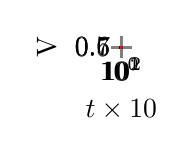
\begin{tikzpicture}

\begin{axis}[%
width=0.951\fwidth,
height=0.75\fwidth,
at={(0\fwidth,0\fwidth)},
scale only axis,
xmode=log,
xmin=1,
xmax=100,
xminorticks=true,
xlabel={$t \times 10$},
ymin=0.45,
ymax=0.7,
ylabel={V},
axis background/.style={fill=white}
]
\addplot [color=blue, line width=2.0pt, forget plot]
  table[row sep=crcr]{%
1	0.457219642968273\\
2	0.592769351348169\\
3	0.628816705720447\\
4	0.62505185351612\\
5	0.628217785699876\\
6	0.639218851111152\\
7	0.630873927371614\\
8	0.636227797683053\\
9	0.638026015044111\\
10	0.636823616047142\\
11	0.632410660316369\\
12	0.633597617267562\\
13	0.636527784056834\\
14	0.637892469025015\\
15	0.633703787028147\\
16	0.636328078671473\\
17	0.637880712599377\\
18	0.634684165215899\\
19	0.629978414138595\\
20	0.628159353629191\\
21	0.637486382196772\\
22	0.630647724209231\\
23	0.636203699395604\\
24	0.632324272807024\\
25	0.643830720098772\\
26	0.633034238724461\\
27	0.635123838924277\\
28	0.636057361395139\\
29	0.642104432395723\\
30	0.63957063775151\\
31	0.636676944667785\\
32	0.638328034343207\\
33	0.642713754763223\\
34	0.638813995795796\\
35	0.637222326954388\\
36	0.641876694490855\\
37	0.637397077631842\\
38	0.641452323880008\\
39	0.639449683802413\\
40	0.63998585281562\\
41	0.645562739043969\\
42	0.638373912813148\\
43	0.63869610092111\\
44	0.639248573866283\\
45	0.64553183974159\\
46	0.64574217834242\\
47	0.647159828876256\\
48	0.642734787921472\\
49	0.645351749272455\\
50	0.647986777824105\\
51	0.648498084835137\\
52	0.641666027891812\\
53	0.649788940171897\\
54	0.644719769480268\\
55	0.642816500136809\\
56	0.648563504192992\\
57	0.647484270514486\\
58	0.646522917641747\\
59	0.646362741362458\\
60	0.64943324763383\\
61	0.650725119238089\\
};
\addplot [color=red, dashed, line width=3.0pt, forget plot]
  table[row sep=crcr]{%
1	0.50533782292246\\
2	0.59699112902373\\
3	0.625888847773672\\
4	0.624084738953654\\
5	0.630607004491168\\
6	0.632831760088705\\
7	0.636757087308418\\
8	0.643065048813731\\
9	0.635831074924727\\
10	0.640172268918583\\
11	0.637618500393285\\
12	0.637063543459606\\
13	0.637801195651245\\
14	0.639132776275881\\
15	0.635237491522697\\
16	0.63711453971561\\
17	0.635829219303754\\
18	0.631722475647075\\
19	0.634325927457996\\
20	0.631533283036592\\
21	0.634408642218423\\
22	0.633190718318277\\
23	0.634003706915972\\
24	0.637844298466811\\
25	0.632637216101121\\
26	0.630133780104625\\
27	0.629845209068525\\
28	0.633468263655565\\
29	0.636356158428604\\
30	0.641203029255701\\
31	0.638991861329888\\
32	0.640709523818283\\
33	0.638816379513034\\
34	0.63827201778754\\
35	0.639309083888535\\
36	0.640322622034011\\
37	0.636038032575251\\
38	0.641624574388145\\
39	0.640674600649206\\
40	0.636610965813643\\
41	0.637518273518509\\
42	0.637490556877938\\
43	0.642085811731694\\
44	0.642900366689167\\
45	0.64514581492819\\
46	0.644982417065964\\
47	0.645169810588366\\
48	0.646840576097694\\
49	0.649222992097267\\
50	0.645768342344984\\
51	0.646975527164982\\
52	0.648342200211879\\
53	0.646810289670806\\
54	0.648718371906363\\
55	0.649127848411779\\
56	0.650500132527732\\
57	0.650312507421561\\
58	0.650414667141449\\
59	0.648262622639421\\
60	0.646204756681934\\
61	0.64655970208432\\
};
\end{axis}
\end{tikzpicture}%
  }
  \subfloat[$\lambda=0.25$]{
    % This file was created by matlab2tikz.
%
%The latest updates can be retrieved from
%  http://www.mathworks.com/matlabcentral/fileexchange/22022-matlab2tikz-matlab2tikz
%where you can also make suggestions and rate matlab2tikz.
%
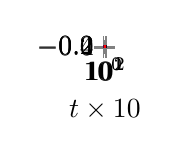
\begin{tikzpicture}

\begin{axis}[%
width=0.951\fwidth,
height=0.75\fwidth,
at={(0\fwidth,0\fwidth)},
scale only axis,
xmode=log,
xmin=1,
xmax=100,
xminorticks=true,
xlabel={$t \times 10$},
ymin=-0.4,
ymax=0.2,
axis background/.style={fill=white}
]
\addplot [color=blue, line width=2.0pt, forget plot]
  table[row sep=crcr]{%
1	-0.107309117160114\\
2	-0.184362598610003\\
3	-0.202687343033588\\
4	-0.16405353282543\\
5	-0.0404647596781372\\
6	-0.142185989426937\\
7	-0.0867070351173507\\
8	-0.103112003957054\\
9	-0.147973876301626\\
10	-0.0559405398752546\\
11	-0.0904189398323078\\
12	-0.143167279778263\\
13	-0.090396490677853\\
14	-0.0933118500216149\\
15	-0.118988174174151\\
16	-0.0678767358522148\\
17	-0.129987246948872\\
18	-0.186594510932254\\
19	-0.0215939023932779\\
20	-0.104510953104091\\
21	-0.13723838749799\\
22	-0.18620095487661\\
23	-0.212719706095191\\
24	-0.225196694541515\\
25	-0.113776632704301\\
26	-0.143391389100894\\
27	-0.243940532329244\\
28	-0.125244153045619\\
29	-0.266760554277998\\
30	-0.275116708400049\\
31	-0.219899848624522\\
32	-0.218521639522065\\
33	-0.221299282448636\\
34	-0.233220662963895\\
35	-0.209380517899935\\
36	-0.236064029388241\\
37	-0.212863027765073\\
38	-0.201394889444524\\
39	-0.237944741868967\\
40	-0.259988067335625\\
41	-0.212928270520192\\
42	-0.279107144092697\\
43	-0.247823881984387\\
44	-0.244473723197659\\
45	-0.27712897889869\\
46	-0.2939114684982\\
47	-0.262173085855822\\
48	-0.224572653789633\\
49	-0.277207371017433\\
50	-0.264808868869637\\
51	-0.255175102937293\\
52	-0.29510233737979\\
53	-0.284122136547406\\
54	-0.243506723452448\\
55	-0.263471235968001\\
56	-0.273090002692023\\
57	-0.282418540838345\\
58	-0.252055818552359\\
59	-0.258663444499106\\
60	-0.291293216722242\\
61	-0.229192294502873\\
};
\addplot [color=red, dashed, line width=3.0pt, forget plot]
  table[row sep=crcr]{%
1	0.156154700909796\\
2	-0.202529646913159\\
3	-0.334501624221845\\
4	-0.318155142166199\\
5	-0.153483607896056\\
6	-0.207611067782485\\
7	-0.185766432059466\\
8	-0.267942726423269\\
9	-0.230990254470568\\
10	-0.187853728223043\\
11	-0.207663739985019\\
12	-0.248003162170955\\
13	-0.226471600713461\\
14	-0.235871101675925\\
15	-0.286725135969644\\
16	-0.264493187308551\\
17	-0.253062643392712\\
18	-0.27076819747302\\
19	-0.241941070940066\\
20	-0.259674995051562\\
21	-0.261194466691931\\
22	-0.243502937063522\\
23	-0.258896757797132\\
24	-0.229200967686043\\
25	-0.243544823178511\\
26	-0.246523459323759\\
27	-0.239579465861304\\
28	-0.2058848765737\\
29	-0.244769717827798\\
30	-0.277044962490945\\
31	-0.261511328888575\\
32	-0.261486322591778\\
33	-0.261059257567426\\
34	-0.240391853350955\\
35	-0.209165659984946\\
36	-0.215611668997483\\
37	-0.219133607027449\\
38	-0.240239168432912\\
39	-0.26495817875911\\
40	-0.290806207461142\\
41	-0.271959186404205\\
42	-0.268198074806926\\
43	-0.26509097620102\\
44	-0.324057188614507\\
45	-0.32565688601495\\
46	-0.311684764206851\\
47	-0.333186997244714\\
48	-0.27544649692533\\
49	-0.250408797980645\\
50	-0.261630623670323\\
51	-0.250494309595537\\
52	-0.258998661381812\\
53	-0.277524904868859\\
54	-0.290114185134193\\
55	-0.268412694296168\\
56	-0.268939296683932\\
57	-0.267282191301071\\
58	-0.271482157224587\\
59	-0.272799271069239\\
60	-0.255638700719698\\
61	-0.255788000793323\\
};
\end{axis}
\end{tikzpicture}%
  }
  \subfloat[$\lambda=0.5$]{
    % This file was created by matlab2tikz.
%
%The latest updates can be retrieved from
%  http://www.mathworks.com/matlabcentral/fileexchange/22022-matlab2tikz-matlab2tikz
%where you can also make suggestions and rate matlab2tikz.
%
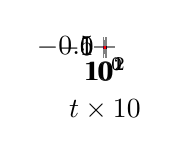
\begin{tikzpicture}

\begin{axis}[%
width=0.951\fwidth,
height=0.75\fwidth,
at={(0\fwidth,0\fwidth)},
scale only axis,
xmode=log,
xmin=1,
xmax=100,
xminorticks=true,
xlabel={$t \times 10$},
ymin=-1.4,
ymax=0,
axis background/.style={fill=white}
]
\addplot [color=blue, line width=2.0pt, forget plot]
  table[row sep=crcr]{%
1	-1.09622117340752\\
2	-0.439738831631238\\
3	-0.477010262732245\\
4	-0.459566994825697\\
5	-0.267438768251134\\
6	-0.261884198822098\\
7	-0.314800806678737\\
8	-0.323934739140698\\
9	-0.204202454295437\\
10	-0.220866546747302\\
11	-0.224784320984486\\
12	-0.174850401323677\\
13	-0.204336810453115\\
14	-0.279220020694667\\
15	-0.304215110722433\\
16	-0.111899168962922\\
17	-0.196698433914746\\
18	-0.212212607848973\\
19	-0.234718297036081\\
20	-0.322668180703975\\
21	-0.286071421580403\\
22	-0.259499649273306\\
23	-0.316375891732036\\
24	-0.273840483206877\\
25	-0.355624719979204\\
26	-0.379757992540423\\
27	-0.288379194513057\\
28	-0.259927407512447\\
29	-0.331340818267421\\
30	-0.342494252379114\\
31	-0.343352143939611\\
32	-0.415313928296665\\
33	-0.422017029459941\\
34	-0.335179784452087\\
35	-0.440060447624601\\
36	-0.514029990888593\\
37	-0.43325890065029\\
38	-0.381527909556519\\
39	-0.357585870240933\\
40	-0.342513238337931\\
41	-0.351232807159593\\
42	-0.491960446194131\\
43	-0.414521352705201\\
44	-0.426725954088604\\
45	-0.442441956965056\\
46	-0.48463572780352\\
47	-0.539087119210198\\
48	-0.444488011314339\\
49	-0.50689510900555\\
50	-0.577616030570053\\
51	-0.438450894005509\\
52	-0.538629948619004\\
53	-0.427097161747581\\
54	-0.449574311025686\\
55	-0.549606168957645\\
56	-0.592101430233288\\
57	-0.633608692550753\\
58	-0.517199531938076\\
59	-0.606102743738442\\
60	-0.513954328614164\\
61	-0.657646711598371\\
};
\addplot [color=red, dashed, line width=3.0pt, forget plot]
  table[row sep=crcr]{%
1	-0.138097439995355\\
2	-0.748893406957869\\
3	-0.82460686564522\\
4	-0.686300787106743\\
5	-0.590927424830682\\
6	-0.644914108373764\\
7	-0.621536393076511\\
8	-0.732227183784745\\
9	-0.678985832465308\\
10	-0.677538882070215\\
11	-0.649492934072179\\
12	-0.626953188541119\\
13	-0.514430272564223\\
14	-0.552610078526062\\
15	-0.651427496731807\\
16	-0.610373827755142\\
17	-0.618730957216695\\
18	-0.62662953336171\\
19	-0.647029602765731\\
20	-0.771071949704786\\
21	-0.881634832338758\\
22	-0.787624432290519\\
23	-0.749027999750425\\
24	-0.768887901516103\\
25	-0.766265274524894\\
26	-0.754819034015115\\
27	-0.682709696959525\\
28	-0.755854713298122\\
29	-0.795893759226808\\
30	-0.87634212964454\\
31	-0.837761717305747\\
32	-0.800158278551069\\
33	-0.788079320268578\\
34	-0.757587585669062\\
35	-0.735977528675732\\
36	-0.792743783163313\\
37	-0.826465829671237\\
38	-0.79949075466688\\
39	-0.763326650871933\\
40	-0.812995026125147\\
41	-0.841258496638301\\
42	-0.811392209795322\\
43	-0.925172456274953\\
44	-0.981952927632142\\
45	-0.903004676499468\\
46	-0.985923064692685\\
47	-1.00004897431729\\
48	-0.981936952406439\\
49	-0.955363797496084\\
50	-0.95804465183494\\
51	-1.02561492499815\\
52	-1.00549051871228\\
53	-0.993986917287425\\
54	-1.03469402307911\\
55	-1.0713271054811\\
56	-1.11079025820582\\
57	-1.12157352569169\\
58	-1.13388551393297\\
59	-1.10161020503734\\
60	-1.10864470943151\\
61	-1.03972034327087\\
};
\end{axis}
\end{tikzpicture}%
  }
  \\
  \subfloat[$\lambda=0.75$]{
    % This file was created by matlab2tikz.
%
%The latest updates can be retrieved from
%  http://www.mathworks.com/matlabcentral/fileexchange/22022-matlab2tikz-matlab2tikz
%where you can also make suggestions and rate matlab2tikz.
%
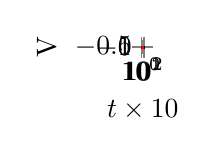
\begin{tikzpicture}

\begin{axis}[%
width=0.951\fwidth,
height=0.75\fwidth,
at={(0\fwidth,0\fwidth)},
scale only axis,
xmode=log,
xmin=1,
xmax=100,
xminorticks=true,
xlabel={$t \times 10$},
ymin=-1.4,
ymax=-0,
ylabel={V},
axis background/.style={fill=white}
]
\addplot [color=blue, line width=2.0pt, forget plot]
  table[row sep=crcr]{%
1	-0.577093123554267\\
2	-0.248954758659022\\
3	-0.35764860428935\\
4	-0.384489263771175\\
5	-0.137724767472587\\
6	-0.287617263649582\\
7	-0.238022447402015\\
8	-0.227177403202236\\
9	-0.167308886039736\\
10	-0.161376703486556\\
11	-0.244705523926808\\
12	-0.225120239981884\\
13	-0.207276792295031\\
14	-0.171776517037101\\
15	-0.172712713325723\\
16	-0.185088779203056\\
17	-0.167798962290238\\
18	-0.164028130972016\\
19	-0.203935674606876\\
20	-0.229890198812524\\
21	-0.206840332491921\\
22	-0.238091646259464\\
23	-0.175086145068783\\
24	-0.256161743484268\\
25	-0.191277333731401\\
26	-0.211347306437156\\
27	-0.19898722167119\\
28	-0.208658653631961\\
29	-0.259816824867176\\
30	-0.237928172498554\\
31	-0.23358861416853\\
32	-0.316512017404449\\
33	-0.204916004601392\\
34	-0.239785151677314\\
35	-0.285154711351199\\
36	-0.201371426057616\\
37	-0.279393824605483\\
38	-0.236736659060055\\
39	-0.258409042059961\\
40	-0.212586736782501\\
41	-0.366452766032414\\
42	-0.225163197594042\\
43	-0.400058658771094\\
44	-0.254925092948163\\
45	-0.283929055975851\\
46	-0.288689458039081\\
47	-0.303848260007582\\
48	-0.306914990520981\\
49	-0.299002998751941\\
50	-0.259695035886033\\
51	-0.320960950250418\\
52	-0.291040251313417\\
53	-0.354678279092358\\
54	-0.226764497936105\\
55	-0.406969528769398\\
56	-0.35735127127503\\
57	-0.450091430573555\\
58	-0.384435368648727\\
59	-0.344316593562978\\
60	-0.342268282505291\\
61	-0.356751765642486\\
};
\addplot [color=red, dashed, line width=3.0pt, forget plot]
  table[row sep=crcr]{%
1	-0.558867096944863\\
2	-1.09288402759395\\
3	-0.839601895925869\\
4	-1.13434859230935\\
5	-0.938751243985718\\
6	-1.02852382062057\\
7	-0.815833675753988\\
8	-1.05133374684411\\
9	-0.880020524351822\\
10	-0.710895330347298\\
11	-0.757053571799602\\
12	-0.693359796897153\\
13	-0.609044947073203\\
14	-0.619878551256528\\
15	-0.770333297321465\\
16	-0.745953732884505\\
17	-0.752773746980868\\
18	-0.842252441020057\\
19	-0.844781239988941\\
20	-0.999171417591342\\
21	-1.15237330771864\\
22	-1.01314018000917\\
23	-0.939869183249194\\
24	-0.82712673891788\\
25	-0.828311262541784\\
26	-0.773600331997152\\
27	-0.745596732067385\\
28	-0.841592443963456\\
29	-0.921138544961516\\
30	-1.02085899320577\\
31	-0.928805249697245\\
32	-0.87047255661201\\
33	-0.86578428332466\\
34	-0.821524625735823\\
35	-0.802852201942028\\
36	-0.869243511936604\\
37	-0.857984019399831\\
38	-0.789458059808354\\
39	-0.729281534798616\\
40	-0.84646490496439\\
41	-0.772860543050829\\
42	-0.79444912383881\\
43	-0.850558520633302\\
44	-0.943529592739689\\
45	-0.911562918124687\\
46	-0.953111291385843\\
47	-1.00327605127269\\
48	-1.02712018838934\\
49	-1.00136473675006\\
50	-1.01619500858576\\
51	-1.16391263914022\\
52	-1.20232686441201\\
53	-1.09666354315773\\
54	-1.16203449202619\\
55	-1.15049813617522\\
56	-1.15281503321226\\
57	-1.21027496105179\\
58	-1.15787421113916\\
59	-1.28995903552509\\
60	-1.21658911309429\\
61	-1.13001821316672\\
};
\end{axis}
\end{tikzpicture}%
  }
  \subfloat[$\lambda=1$]{
    % This file was created by matlab2tikz.
%
%The latest updates can be retrieved from
%  http://www.mathworks.com/matlabcentral/fileexchange/22022-matlab2tikz-matlab2tikz
%where you can also make suggestions and rate matlab2tikz.
%
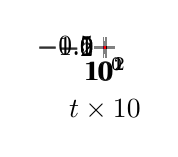
\begin{tikzpicture}

\begin{axis}[%
width=0.951\fwidth,
height=0.75\fwidth,
at={(0\fwidth,0\fwidth)},
scale only axis,
xmode=log,
xmin=1,
xmax=100,
xminorticks=true,
xlabel={$t \times 10$},
ymin=-2,
ymax=-0,
axis background/.style={fill=white}
]
\addplot [color=blue, line width=2.0pt, forget plot]
  table[row sep=crcr]{%
1	-0.00232770753700901\\
2	-1.97313695873102e-05\\
3	-2.37767934892516e-06\\
4	-5.41730805759902e-07\\
5	-7.32149168349694e-08\\
6	-2.39811834130854e-08\\
7	-5.18082968701592e-09\\
8	-5.80788316935145e-09\\
9	-1.76256829256548e-09\\
10	-1.38567073595432e-09\\
11	-2.7766696901406e-10\\
12	-2.3480673996106e-10\\
13	-8.92285754128819e-11\\
14	-1.19961233710043e-10\\
15	-2.67771625177127e-11\\
16	-2.1807283694217e-11\\
17	-9.888893758119e-12\\
18	-2.04587275550225e-11\\
19	-1.00294880288958e-11\\
20	-7.27273007814714e-12\\
21	-2.18409079376077e-12\\
22	-1.90552725474449e-12\\
23	-3.08552681136802e-12\\
24	-1.04407443807789e-12\\
25	-6.89534351010657e-13\\
26	-7.04452116553748e-13\\
27	-5.33265371320719e-13\\
28	-2.21733300835158e-13\\
29	-1.09917521624577e-13\\
30	-1.97092353458009e-13\\
31	-1.06901072975012e-13\\
32	-1.02563119096526e-13\\
33	-8.84436177317179e-14\\
34	-3.79100124163196e-14\\
35	-4.2067887937253e-14\\
36	-2.70027547549659e-14\\
37	-2.66635307650848e-14\\
38	-2.67287785600447e-14\\
39	-2.64342999326352e-14\\
40	-2.65179986462852e-14\\
41	-2.68229872585042e-14\\
42	-2.66997278710527e-14\\
43	-2.69707767201082e-14\\
44	-2.67044068810534e-14\\
45	-2.67210612428623e-14\\
46	-2.65715988911875e-14\\
47	-2.65002787170287e-14\\
48	-2.64873004782108e-14\\
49	-2.61218989350948e-14\\
50	-2.64084264642284e-14\\
51	-2.65721748735916e-14\\
52	-2.66424481150276e-14\\
53	-2.65125945760817e-14\\
54	-2.61390327175519e-14\\
55	-2.63298827930954e-14\\
56	-2.66575354658841e-14\\
57	-2.65806977191069e-14\\
58	-2.63970270948243e-14\\
59	-2.63521868646625e-14\\
60	-2.62708242678811e-14\\
61	-2.67337836777301e-14\\
};
\addplot [color=red, dashed, line width=3.0pt, forget plot]
  table[row sep=crcr]{%
1	-1.61749222996759\\
2	-0.501016985730073\\
3	-0.230141055920469\\
4	-0.211363679210412\\
5	-0.180351722603156\\
6	-0.199490315348852\\
7	-0.167503225130075\\
8	-0.197680427138255\\
9	-0.168326964955281\\
10	-0.108154945624742\\
11	-0.121796007045675\\
12	-0.123244092080481\\
13	-0.120059074298961\\
14	-0.12768082663036\\
15	-0.118695747205944\\
16	-0.14620525838291\\
17	-0.156154755993665\\
18	-0.15210970699618\\
19	-0.171018095781681\\
20	-0.159637204861449\\
21	-0.147168529193469\\
22	-0.282154360398568\\
23	-0.245469097598784\\
24	-0.252947839856794\\
25	-0.242482705863201\\
26	-0.244915288625687\\
27	-0.224359689620484\\
28	-0.214533978554422\\
29	-0.216114585568234\\
30	-0.208860180236654\\
31	-0.221529291908727\\
32	-0.205563531932023\\
33	-0.233055721377914\\
34	-0.23298981535382\\
35	-0.215062245554676\\
36	-0.226954153936872\\
37	-0.222039885512241\\
38	-0.198543948266946\\
39	-0.191065849011378\\
40	-0.189777971418282\\
41	-0.188793398961995\\
42	-0.190732460573578\\
43	-0.185246409681183\\
44	-0.184603807555449\\
45	-0.188647955865062\\
46	-0.191033781025243\\
47	-0.179745728112148\\
48	-0.178803266307534\\
49	-0.163926246089407\\
50	-0.173423292392264\\
51	-0.179302094659936\\
52	-0.181333239906458\\
53	-0.177046092214897\\
54	-0.184951112414626\\
55	-0.181338109208384\\
56	-0.147815635344293\\
57	-0.149881515239679\\
58	-0.14463523042435\\
59	-0.144488753661275\\
60	-0.150296785419916\\
61	-0.157708726945062\\
};
\end{axis}
\end{tikzpicture}%
  }
  \subfloat[legend]{
    \raisebox{4em}{\begin{tikzpicture}

  \begin{axis}[%
    hide axis,
    xmin=10,
    xmax=50,
    ymin=0,
    ymax=0.4,
    legend style={draw=white!15!black,legend cell align=left}
    ]
    \addlegendimage{color=mycolor1, line width=2.0pt}
    \addlegendentry{Bayes};
    \addlegendimage{color=mycolor2, dashed, line width=3.0pt};
    \addlegendentry{Marginal};
  \end{axis}
\end{tikzpicture}
}
  }

  \caption{\textbf{COMPAS dataset.} Demonstration of balance on the COMPAS dataset. The plots show the value measured on the holdout set for the \textbf{Bayes} and \textbf{Marginal} balance.
  Figures (a-e) show the utility achieved under different choices of $\lambda$ as we we observe each of the  6,000 training data points. Utility and fairness are measured on the empirical distribution of the remaining data and it can be seen that the Bayesian approach dominates as soon as fairness becomes important, i.e. $\lambda > 0$.  }
  \label{fig:compas-dbn_extend}
\end{figure*}


\begin{figure*}
\centering
  \subfloat[$\lambda=0$]{
    % This file was created by matlab2tikz.
%
%The latest updates can be retrieved from
%  http://www.mathworks.com/matlabcentral/fileexchange/22022-matlab2tikz-matlab2tikz
%where you can also make suggestions and rate matlab2tikz.
%
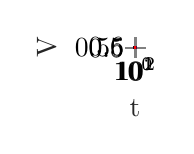
\begin{tikzpicture}

\begin{axis}[%
width=0.951\fwidth,
height=0.75\fwidth,
at={(0\fwidth,0\fwidth)},
scale only axis,
xmode=log,
xmin=1,
xmax=100,
xminorticks=true,
xlabel style={font=\color{white!15!black}},
xlabel={t},
ymin=0.5,
ymax=0.64,
ylabel style={font=\color{white!15!black}},
ylabel={V},
axis background/.style={fill=white}
]
\addplot [color=blue, line width=2.0pt, forget plot]
  table[row sep=crcr]{%
1	0.533404412801252\\
2	0.567059367237681\\
3	0.574983684728794\\
4	0.595440941591605\\
5	0.597329784902714\\
6	0.598376899476387\\
7	0.608381899604062\\
8	0.614299903055019\\
9	0.614682328515722\\
10	0.622047920597586\\
11	0.624110283420211\\
12	0.623040076545587\\
13	0.622922815525939\\
14	0.622693703044924\\
15	0.624972493335543\\
16	0.623768267741923\\
17	0.625076223581217\\
18	0.624417108492841\\
19	0.624469368091222\\
20	0.626122024040929\\
21	0.627990230164747\\
22	0.627328710101433\\
23	0.627229984116765\\
24	0.627284500665436\\
25	0.628167660760683\\
26	0.62745907557843\\
27	0.627233400174376\\
28	0.626561170176999\\
29	0.626140421275828\\
30	0.627206627096838\\
31	0.626985313402765\\
32	0.627098543124935\\
33	0.626653517790801\\
34	0.62669323165553\\
35	0.626164136918594\\
36	0.625226096500675\\
37	0.624375614738648\\
38	0.626043052672986\\
39	0.625037401619658\\
40	0.624754173295781\\
41	0.625734326489491\\
42	0.624858959455676\\
43	0.624748862220927\\
44	0.625474170196668\\
45	0.624772055502031\\
46	0.624434789925371\\
47	0.624134265867323\\
48	0.624465786011358\\
49	0.62488377850369\\
50	0.624799243863898\\
51	0.623188769161788\\
52	0.622787015457619\\
53	0.625093107691527\\
54	0.62416250160529\\
55	0.624845855606283\\
56	0.625039701294087\\
57	0.625218860435963\\
58	0.626623043783051\\
59	0.626765171689463\\
60	0.626873002508487\\
};
\addplot [color=red, dashed, line width=3.0pt, forget plot]
  table[row sep=crcr]{%
1	0.537691550449067\\
2	0.52692425944197\\
3	0.51952806147473\\
4	0.516060917995437\\
5	0.525734464151558\\
6	0.526857982759685\\
7	0.527688486772251\\
8	0.553006242367054\\
9	0.580639537966924\\
10	0.583055435798432\\
11	0.583845485337254\\
12	0.585535021854244\\
13	0.589716220033718\\
14	0.591727972382982\\
15	0.592321109916687\\
16	0.593212336283605\\
17	0.59331788850473\\
18	0.592639117087132\\
19	0.594276492899578\\
20	0.593631864589812\\
21	0.593134373439542\\
22	0.592526975573227\\
23	0.59343823978082\\
24	0.59471503376963\\
25	0.594382031634667\\
26	0.59347186036185\\
27	0.594295880998185\\
28	0.592974355499971\\
29	0.594610054709994\\
30	0.594316274450942\\
31	0.59587687254927\\
32	0.594384171167264\\
33	0.59368169358206\\
34	0.593672061191477\\
35	0.59309575835021\\
36	0.591830149985295\\
37	0.592248365155305\\
38	0.592785655298101\\
39	0.592284775003569\\
40	0.591763395381349\\
41	0.591416781456517\\
42	0.593000957180953\\
43	0.591369641506618\\
44	0.592580298295271\\
45	0.592677941655292\\
46	0.591707641469623\\
47	0.592929785718232\\
48	0.591688464121018\\
49	0.591343754331541\\
50	0.589724575501398\\
51	0.590358577218326\\
52	0.590327436945083\\
53	0.590665615799822\\
54	0.595774337247164\\
55	0.595592315397091\\
56	0.595804057900644\\
57	0.59578874458756\\
58	0.596457066440588\\
59	0.597530717491227\\
60	0.597648444447298\\
};
\end{axis}
\end{tikzpicture}%
  }
  \subfloat[$\lambda=0.25$]{
    % This file was created by matlab2tikz.
%
%The latest updates can be retrieved from
%  http://www.mathworks.com/matlabcentral/fileexchange/22022-matlab2tikz-matlab2tikz
%where you can also make suggestions and rate matlab2tikz.
%
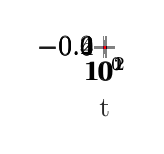
\begin{tikzpicture}

\begin{axis}[%
width=0.951\fwidth,
height=0.75\fwidth,
at={(0\fwidth,0\fwidth)},
scale only axis,
xmode=log,
xmin=1,
xmax=100,
xminorticks=true,
xlabel style={font=\color{white!15!black}},
xlabel={t},
ymin=-0.7,
ymax=0.1,
axis background/.style={fill=white}
]
\addplot [color=blue, line width=2.0pt, forget plot]
  table[row sep=crcr]{%
1	-0.207196320566641\\
2	-0.425253875761661\\
3	-0.446970299122139\\
4	-0.41023006864754\\
5	-0.373322872219761\\
6	-0.367076094492257\\
7	-0.412878957537136\\
8	-0.413231937902242\\
9	-0.396049100003292\\
10	-0.373751675886177\\
11	-0.307771466008203\\
12	-0.142776108558127\\
13	-0.0925268949955039\\
14	-0.043827489725773\\
15	-0.0362719426975273\\
16	-0.0534966546269057\\
17	-0.0470706573695844\\
18	-0.0439917899143233\\
19	-0.0731027476537716\\
20	-0.0710715562201365\\
21	0.0127395664509126\\
22	0.0125535248449869\\
23	-0.0189231624399058\\
24	-0.0277232488542588\\
25	-0.0134581577090796\\
26	-0.0217588559150046\\
27	-0.0216893000684138\\
28	-0.0301266863372562\\
29	-0.0423852719635449\\
30	-0.0837378934262495\\
31	-0.0752088135448239\\
32	-0.0701158205484715\\
33	-0.0550343965029364\\
34	-0.0598645896360828\\
35	-0.0535803870353569\\
36	-0.0486584450371605\\
37	-0.0528834512409008\\
38	-0.09374799126579\\
39	-0.108641858592263\\
40	-0.116196652395813\\
41	-0.116755534241694\\
42	-0.0790210057246608\\
43	-0.101120407287318\\
44	-0.119825974775341\\
45	-0.114650814449016\\
46	-0.127224682409873\\
47	-0.15229978166135\\
48	-0.150131385782543\\
49	-0.158781774372714\\
50	-0.15623051925632\\
51	-0.167159607725622\\
52	-0.192822190369984\\
53	-0.187108430802122\\
54	-0.181673668158932\\
55	-0.208850712289315\\
56	-0.2069069917245\\
57	-0.211187039445116\\
58	-0.20459968944502\\
59	-0.190336379312404\\
60	-0.193366570484612\\
};
\addplot [color=red, dashed, line width=3.0pt, forget plot]
  table[row sep=crcr]{%
1	-0.310007172235672\\
2	-0.423714921637176\\
3	-0.410133018536837\\
4	-0.439747920197301\\
5	-0.455407707547421\\
6	-0.498202819436065\\
7	-0.5120224711627\\
8	-0.520697951706963\\
9	-0.523509545840905\\
10	-0.513259555010702\\
11	-0.534619050417941\\
12	-0.524377332258372\\
13	-0.540265530899788\\
14	-0.546714144110614\\
15	-0.557246115736649\\
16	-0.556180713008244\\
17	-0.506115024268118\\
18	-0.452408989176526\\
19	-0.438493393679697\\
20	-0.301299392319608\\
21	-0.143032833276735\\
22	-0.22920493119444\\
23	-0.36646075589015\\
24	-0.294566905747852\\
25	-0.243896037045222\\
26	-0.26842926302992\\
27	-0.276511738663329\\
28	-0.334838492474182\\
29	-0.36257984378723\\
30	-0.363663238136526\\
31	-0.377404312691054\\
32	-0.339176332999594\\
33	-0.316367727873905\\
34	-0.0775681732383819\\
35	-0.115417577113182\\
36	-0.174373859692571\\
37	-0.0543473840941811\\
38	-0.0646683542813737\\
39	-0.0736473944879555\\
40	-0.108832687588216\\
41	-0.153868009813003\\
42	-0.148133426159907\\
43	-0.191274332541181\\
44	-0.207928678469066\\
45	-0.206719417210556\\
46	-0.189150556247738\\
47	-0.20885630192149\\
48	-0.179619375326677\\
49	-0.196970384143575\\
50	-0.192503247410312\\
51	-0.237320806979659\\
52	-0.226844801344638\\
53	-0.261983151124036\\
54	-0.288565282674517\\
55	-0.298741252764581\\
56	-0.301494430295086\\
57	-0.296720140763373\\
58	-0.287235205015912\\
59	-0.278661589789526\\
60	-0.283053655854063\\
};
\end{axis}
\end{tikzpicture}%
  }
  \subfloat[$\lambda=0.5$]{
    % This file was created by matlab2tikz.
%
%The latest updates can be retrieved from
%  http://www.mathworks.com/matlabcentral/fileexchange/22022-matlab2tikz-matlab2tikz
%where you can also make suggestions and rate matlab2tikz.
%
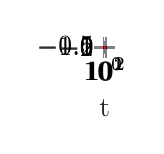
\begin{tikzpicture}

\begin{axis}[%
width=0.951\fwidth,
height=0.75\fwidth,
at={(0\fwidth,0\fwidth)},
scale only axis,
xmode=log,
xmin=1,
xmax=100,
xminorticks=true,
xlabel style={font=\color{white!15!black}},
xlabel={t},
ymin=-2,
ymax=-0,
axis background/.style={fill=white}
]
\addplot [color=blue, line width=2.0pt, forget plot]
  table[row sep=crcr]{%
1	-0.139557730363354\\
2	-0.238920667169255\\
3	-0.0997916326764938\\
4	-0.182229548458017\\
5	-0.205267446075831\\
6	-0.279826712648142\\
7	-0.332249305176689\\
8	-0.323237535828966\\
9	-0.334848601807552\\
10	-0.312990041492882\\
11	-0.324619975130561\\
12	-0.328870423071226\\
13	-0.313326571427902\\
14	-0.319808076558834\\
15	-0.30709006893331\\
16	-0.317914410723469\\
17	-0.331045983578041\\
18	-0.342385254226511\\
19	-0.358246869022327\\
20	-0.369248314322897\\
21	-0.377973473224499\\
22	-0.415440383538921\\
23	-0.38990705668132\\
24	-0.36686729244785\\
25	-0.375042658748737\\
26	-0.366006828119552\\
27	-0.383213880975782\\
28	-0.386114407046102\\
29	-0.380250046047834\\
30	-0.399759884881641\\
31	-0.437509783568944\\
32	-0.439357807489347\\
33	-0.443493819937183\\
34	-0.43823346019647\\
35	-0.448743781654721\\
36	-0.46057428729186\\
37	-0.465056676021326\\
38	-0.455095054216753\\
39	-0.463602980734887\\
40	-0.497134299702848\\
41	-0.456405475996486\\
42	-0.461607953659762\\
43	-0.467431543238734\\
44	-0.481699178907957\\
45	-0.497488409531242\\
46	-0.491566651303831\\
47	-0.489462737779279\\
48	-0.508962806633321\\
49	-0.497498682067592\\
50	-0.49354033957002\\
51	-0.497912056057912\\
52	-0.496093017678467\\
53	-0.505412512936155\\
54	-0.503382028933859\\
55	-0.52416214442533\\
56	-0.522603926762207\\
57	-0.544550008258789\\
58	-0.532153628446791\\
59	-0.520440892587704\\
60	-0.532834541878595\\
};
\addplot [color=red, dashed, line width=3.0pt, forget plot]
  table[row sep=crcr]{%
1	-0.759593109224573\\
2	-0.851910476827388\\
3	-0.931248398068395\\
4	-0.899099878562075\\
5	-0.7313280766324\\
6	-0.866207448068707\\
7	-0.990998285997023\\
8	-1.0272085536674\\
9	-1.04372995832914\\
10	-1.07714261034557\\
11	-1.07998626920429\\
12	-1.1166916978057\\
13	-1.09921640121892\\
14	-1.11870116207787\\
15	-1.14149626270435\\
16	-1.13602637450519\\
17	-1.19256259507435\\
18	-1.18855636890274\\
19	-1.16210813506113\\
20	-1.19312997954371\\
21	-1.16517236023971\\
22	-1.09072259193678\\
23	-1.07693553149219\\
24	-1.09320599058905\\
25	-1.12532578022789\\
26	-1.14329006175479\\
27	-1.17276265772882\\
28	-1.15208234230952\\
29	-1.18083392582687\\
30	-1.20703772222562\\
31	-1.22005481633382\\
32	-1.21874241865254\\
33	-1.26208489068812\\
34	-1.22937949908594\\
35	-1.26117480001724\\
36	-1.2690068818918\\
37	-1.26700389402755\\
38	-1.27433797411748\\
39	-1.28632957244659\\
40	-1.31543453440127\\
41	-1.32705144995612\\
42	-1.33602820271486\\
43	-1.3294527996667\\
44	-1.31996093710498\\
45	-1.32018176557428\\
46	-1.32494053379554\\
47	-1.33735592039034\\
48	-1.34339401770564\\
49	-1.33957969692087\\
50	-1.35053901850318\\
51	-1.34476886404259\\
52	-1.37641480485034\\
53	-1.35196334938376\\
54	-1.38384298807204\\
55	-1.40343614175046\\
56	-1.38977437984097\\
57	-1.37450630646827\\
58	-1.39440827751891\\
59	-1.41230095819747\\
60	-1.42020708154538\\
};
\end{axis}
\end{tikzpicture}%
  }
  \\
  \subfloat[$\lambda=0.75$]{
    % This file was created by matlab2tikz.
%
%The latest updates can be retrieved from
%  http://www.mathworks.com/matlabcentral/fileexchange/22022-matlab2tikz-matlab2tikz
%where you can also make suggestions and rate matlab2tikz.
%
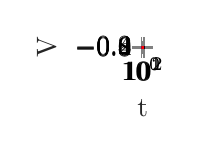
\begin{tikzpicture}

\begin{axis}[%
width=0.951\fwidth,
height=0.75\fwidth,
at={(0\fwidth,0\fwidth)},
scale only axis,
xmode=log,
xmin=1,
xmax=100,
xminorticks=true,
xlabel style={font=\color{white!15!black}},
xlabel={t},
ymin=-0.8,
ymax=-0,
ylabel style={font=\color{white!15!black}},
ylabel={V},
axis background/.style={fill=white}
]
\addplot [color=blue, line width=2.0pt, forget plot]
  table[row sep=crcr]{%
1	-0.0698670388969574\\
2	-0.0961890539986359\\
3	-0.132699144478001\\
4	-0.183101635988515\\
5	-0.250742140214741\\
6	-0.293266160267643\\
7	-0.276102246336143\\
8	-0.293448152823888\\
9	-0.344386347148344\\
10	-0.319149736907851\\
11	-0.297734928600805\\
12	-0.311571017833386\\
13	-0.294400148828445\\
14	-0.302231089798049\\
15	-0.243116324401653\\
16	-0.212083661389009\\
17	-0.233746426259225\\
18	-0.25286643122445\\
19	-0.236721961942786\\
20	-0.227153876544933\\
21	-0.239960732080747\\
22	-0.252464630359502\\
23	-0.221722655206653\\
24	-0.242234634999856\\
25	-0.215727187789023\\
26	-0.207245184391738\\
27	-0.198602366718053\\
28	-0.216362141232685\\
29	-0.203299221987791\\
30	-0.231551022346517\\
31	-0.223148752456014\\
32	-0.223513820452022\\
33	-0.234256655945202\\
34	-0.236933370776921\\
35	-0.266032198231509\\
36	-0.278628900515368\\
37	-0.264393610861771\\
38	-0.274638150183318\\
39	-0.29837283368362\\
40	-0.300363381099991\\
41	-0.302679151560454\\
42	-0.314870541600552\\
43	-0.278041572603173\\
44	-0.305742628530841\\
45	-0.286874359979552\\
46	-0.303919077702958\\
47	-0.328469119416157\\
48	-0.295742198577038\\
49	-0.32463667447715\\
50	-0.312820348014414\\
51	-0.322105149700822\\
52	-0.324641287036458\\
53	-0.297480905675212\\
54	-0.324260928208976\\
55	-0.33325489418501\\
56	-0.341060371144084\\
57	-0.342033707353245\\
58	-0.328434744104012\\
59	-0.330087267902574\\
60	-0.325796950505763\\
};
\addplot [color=red, dashed, line width=3.0pt, forget plot]
  table[row sep=crcr]{%
1	-0.798003405407076\\
2	-0.795088043311391\\
3	-0.748309023109161\\
4	-0.612609627478908\\
5	-0.58164859025222\\
6	-0.427949774021936\\
7	-0.454360176873906\\
8	-0.437345512177144\\
9	-0.402815955453931\\
10	-0.390244257342745\\
11	-0.419601914557706\\
12	-0.440904840008107\\
13	-0.39469526906995\\
14	-0.35483201391564\\
15	-0.353091583286641\\
16	-0.385734545472699\\
17	-0.387596782234304\\
18	-0.406852358977653\\
19	-0.409701930267887\\
20	-0.394138146001548\\
21	-0.417418249782155\\
22	-0.427383645577882\\
23	-0.393622565060579\\
24	-0.382161985890078\\
25	-0.375151768834539\\
26	-0.364797112866392\\
27	-0.397971634740718\\
28	-0.428159932609351\\
29	-0.382225019086256\\
30	-0.410457553255195\\
31	-0.435679219800089\\
32	-0.412057421507584\\
33	-0.441729441705593\\
34	-0.440313423318161\\
35	-0.416706751428254\\
36	-0.418300438155118\\
37	-0.397801980051729\\
38	-0.424732450230448\\
39	-0.437152223855908\\
40	-0.433518092412821\\
41	-0.39931985670458\\
42	-0.435267220777679\\
43	-0.437592218978853\\
44	-0.419300957364138\\
45	-0.416881037406579\\
46	-0.396128656626779\\
47	-0.425764606269481\\
48	-0.438534695701502\\
49	-0.432377081083798\\
50	-0.441463980518391\\
51	-0.444304763034727\\
52	-0.452474923000981\\
53	-0.448621837213215\\
54	-0.42064435309106\\
55	-0.421020067123781\\
56	-0.454665887594057\\
57	-0.465649610557996\\
58	-0.472048153258424\\
59	-0.471067458917294\\
60	-0.448310148007703\\
};
\end{axis}
\end{tikzpicture}%
  }
  \subfloat[$\lambda=1$]{
    % This file was created by matlab2tikz.
%
%The latest updates can be retrieved from
%  http://www.mathworks.com/matlabcentral/fileexchange/22022-matlab2tikz-matlab2tikz
%where you can also make suggestions and rate matlab2tikz.
%
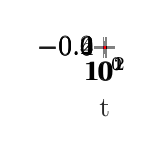
\begin{tikzpicture}

\begin{axis}[%
width=0.951\fwidth,
height=0.75\fwidth,
at={(0\fwidth,0\fwidth)},
scale only axis,
xmode=log,
xmin=1,
xmax=100,
xminorticks=true,
xlabel style={font=\color{white!15!black}},
xlabel={t},
ymin=-0.7,
ymax=-0,
axis background/.style={fill=white}
]
\addplot [color=blue, line width=2.0pt, forget plot]
  table[row sep=crcr]{%
1	-0.015991389253571\\
2	-8.07710251594484e-14\\
3	-2.59936539286564e-14\\
4	-2.60348785986828e-14\\
5	-2.60224200315188e-14\\
6	-2.59820525418944e-14\\
7	-2.59965938614317e-14\\
8	-2.60060611148019e-14\\
9	-2.59506757310226e-14\\
10	-2.58498969706858e-14\\
11	-2.58919987094477e-14\\
12	-2.59483989064604e-14\\
13	-2.595303495495e-14\\
14	-2.59150661948695e-14\\
15	-2.59299891535716e-14\\
16	-2.59070821300713e-14\\
17	-2.58991891382556e-14\\
18	-2.59151399206172e-14\\
19	-2.59036430407802e-14\\
20	-2.59284539232954e-14\\
21	-2.58943058916708e-14\\
22	-2.58760956319817e-14\\
23	-2.59459746304027e-14\\
24	-2.59175295022054e-14\\
25	-2.59825035699981e-14\\
26	-2.58938635371844e-14\\
27	-2.58310058320324e-14\\
28	-2.58420733678091e-14\\
29	-2.58783117412223e-14\\
30	-2.58440162581022e-14\\
31	-2.58429971080601e-14\\
32	-2.58351474843313e-14\\
33	-2.5869000612965e-14\\
34	-2.59091421141991e-14\\
35	-2.58739836061497e-14\\
36	-2.59131536622373e-14\\
37	-2.5829626726869e-14\\
38	-2.58271634195331e-14\\
39	-2.59047142325266e-14\\
40	-2.58443241715192e-14\\
41	-2.58396707757949e-14\\
42	-2.58215472522796e-14\\
43	-2.57845499373457e-14\\
44	-2.57547777456893e-14\\
45	-2.58627556084514e-14\\
46	-2.58798513083072e-14\\
47	-2.58572825558847e-14\\
48	-2.58443111610931e-14\\
49	-2.58880695607746e-14\\
50	-2.60105757326481e-14\\
51	-2.59875602889306e-14\\
52	-2.60626044265013e-14\\
53	-2.58993130083538e-14\\
54	-2.5891459860968e-14\\
55	-2.58690168759975e-14\\
56	-2.59416063798498e-14\\
57	-2.59585459545927e-14\\
58	-2.5878549181498e-14\\
59	-2.57975375951699e-14\\
60	-2.59211019483637e-14\\
};
\addplot [color=red, dashed, line width=3.0pt, forget plot]
  table[row sep=crcr]{%
1	-0.677360003940489\\
2	-0.319188261527385\\
3	-0.238573589451842\\
4	-0.200742996733391\\
5	-0.188801791973792\\
6	-0.157848169305053\\
7	-0.147363581418297\\
8	-0.151590768638053\\
9	-0.164301512639608\\
10	-0.198659955535581\\
11	-0.185472157543024\\
12	-0.189488927671266\\
13	-0.156665545344133\\
14	-0.141346012616817\\
15	-0.142828076379696\\
16	-0.143980205895357\\
17	-0.14494774267628\\
18	-0.145557100703442\\
19	-0.14609092309342\\
20	-0.137324402147981\\
21	-0.134764797162596\\
22	-0.140554448009126\\
23	-0.142899121135694\\
24	-0.143712900049346\\
25	-0.138774590312461\\
26	-0.13836037206626\\
27	-0.135282806601259\\
28	-0.149453779259262\\
29	-0.147470735870606\\
30	-0.154207490480793\\
31	-0.155796490189568\\
32	-0.158732344859596\\
33	-0.163488711963298\\
34	-0.166258826196893\\
35	-0.172242532053593\\
36	-0.168635982124319\\
37	-0.170553091320478\\
38	-0.171303646165357\\
39	-0.185837521836149\\
40	-0.180259389616782\\
41	-0.174263442475532\\
42	-0.162013378918257\\
43	-0.167114368469105\\
44	-0.169568455307836\\
45	-0.173271142995335\\
46	-0.191054413001525\\
47	-0.202850261177353\\
48	-0.209494088522992\\
49	-0.213131370871494\\
50	-0.211058535404276\\
51	-0.207988868337055\\
52	-0.20444195101075\\
53	-0.209951638264728\\
54	-0.218554354326512\\
55	-0.227181804255464\\
56	-0.233332843632866\\
57	-0.240435706083566\\
58	-0.246103352664639\\
59	-0.243526218854078\\
60	-0.236038905669898\\
};
\end{axis}
\end{tikzpicture}%
  }
  \subfloat[legend]{
    \raisebox{4em}{\begin{tikzpicture}

  \begin{axis}[%
    hide axis,
    xmin=10,
    xmax=50,
    ymin=0,
    ymax=0.4,
    legend style={draw=white!15!black,legend cell align=left}
    ]
    \addlegendimage{color=mycolor1, line width=2.0pt}
    \addlegendentry{Bayes};
    \addlegendimage{color=mycolor2, dashed, line width=3.0pt};
    \addlegendentry{Marginal};
  \end{axis}
\end{tikzpicture}
}
  }
\caption{\textbf{Sequential allocation.} Performance measured with respect to the empirical model of the holdout COMPAS data, when the DM's actions affect which data will be seen. This means that wif a prisoner was not released, then the dependent variable $y$ will remain unseen. For that reason, the performance of the Bayesian approach dominates the classical approach even when fairness is not an issue, i.e. $\lambda = 0$.}
\label{fig:sequential-allocation_extend}
\end{figure*}





%\section{Proof of Lemma \ref{lemma:ult}}
%\begin{proof}
%  Let $a^*(x) \defn \max_a \E(\util \mid a, x)$ for some arbitrary
%  distribution. Then for any randomized policy $\pol$:
%  \begin{align*}
%  &\E^\pol(\util \mid x) =
%  \int_{\CA} \E(\util \mid a, x) \dd \pol(a \mid x)\\
%  &\leq \int_{\CA} \E(\util \mid a^*, x) \dd \pol(a \mid x)\\
%  &=\E(\util \mid a^*, x) \dd \pol(a \mid x).
%  \end{align*} 
%  We first apply this to the distribution $\bel(\param)$ to obtain the
%  result for Thompson sampling. For stochastic dominance, note that
%  $$\Pr_\bel(X > Y) = \int_\Param \Pr_\param(X > Y) \dd \bel(\param).$$
%  As stochastic dominance can be implemented by first sampling a
%  parameter and then sampling a dominant variable under this
%  parameter, we can reapply this fact and obtain the final result.
%\end{proof}
%%% Local Variables:
%%% mode: latex
%%% TeX-master: "subjective-fairness"
%%% End:
